% Options for packages loaded elsewhere
\PassOptionsToPackage{unicode}{hyperref}
\PassOptionsToPackage{hyphens}{url}
%
\documentclass[
]{article}
\usepackage{amsmath,amssymb}
\usepackage{lmodern}
\usepackage{iftex}
\ifPDFTeX
  \usepackage[T1]{fontenc}
  \usepackage[utf8]{inputenc}
  \usepackage{textcomp} % provide euro and other symbols
\else % if luatex or xetex
  \usepackage{unicode-math}
  \defaultfontfeatures{Scale=MatchLowercase}
  \defaultfontfeatures[\rmfamily]{Ligatures=TeX,Scale=1}
\fi
% Use upquote if available, for straight quotes in verbatim environments
\IfFileExists{upquote.sty}{\usepackage{upquote}}{}
\IfFileExists{microtype.sty}{% use microtype if available
  \usepackage[]{microtype}
  \UseMicrotypeSet[protrusion]{basicmath} % disable protrusion for tt fonts
}{}
\makeatletter
\@ifundefined{KOMAClassName}{% if non-KOMA class
  \IfFileExists{parskip.sty}{%
    \usepackage{parskip}
  }{% else
    \setlength{\parindent}{0pt}
    \setlength{\parskip}{6pt plus 2pt minus 1pt}}
}{% if KOMA class
  \KOMAoptions{parskip=half}}
\makeatother
\usepackage{xcolor}
\usepackage[margin=1in]{geometry}
\usepackage{color}
\usepackage{fancyvrb}
\newcommand{\VerbBar}{|}
\newcommand{\VERB}{\Verb[commandchars=\\\{\}]}
\DefineVerbatimEnvironment{Highlighting}{Verbatim}{commandchars=\\\{\}}
% Add ',fontsize=\small' for more characters per line
\usepackage{framed}
\definecolor{shadecolor}{RGB}{248,248,248}
\newenvironment{Shaded}{\begin{snugshade}}{\end{snugshade}}
\newcommand{\AlertTok}[1]{\textcolor[rgb]{0.94,0.16,0.16}{#1}}
\newcommand{\AnnotationTok}[1]{\textcolor[rgb]{0.56,0.35,0.01}{\textbf{\textit{#1}}}}
\newcommand{\AttributeTok}[1]{\textcolor[rgb]{0.77,0.63,0.00}{#1}}
\newcommand{\BaseNTok}[1]{\textcolor[rgb]{0.00,0.00,0.81}{#1}}
\newcommand{\BuiltInTok}[1]{#1}
\newcommand{\CharTok}[1]{\textcolor[rgb]{0.31,0.60,0.02}{#1}}
\newcommand{\CommentTok}[1]{\textcolor[rgb]{0.56,0.35,0.01}{\textit{#1}}}
\newcommand{\CommentVarTok}[1]{\textcolor[rgb]{0.56,0.35,0.01}{\textbf{\textit{#1}}}}
\newcommand{\ConstantTok}[1]{\textcolor[rgb]{0.00,0.00,0.00}{#1}}
\newcommand{\ControlFlowTok}[1]{\textcolor[rgb]{0.13,0.29,0.53}{\textbf{#1}}}
\newcommand{\DataTypeTok}[1]{\textcolor[rgb]{0.13,0.29,0.53}{#1}}
\newcommand{\DecValTok}[1]{\textcolor[rgb]{0.00,0.00,0.81}{#1}}
\newcommand{\DocumentationTok}[1]{\textcolor[rgb]{0.56,0.35,0.01}{\textbf{\textit{#1}}}}
\newcommand{\ErrorTok}[1]{\textcolor[rgb]{0.64,0.00,0.00}{\textbf{#1}}}
\newcommand{\ExtensionTok}[1]{#1}
\newcommand{\FloatTok}[1]{\textcolor[rgb]{0.00,0.00,0.81}{#1}}
\newcommand{\FunctionTok}[1]{\textcolor[rgb]{0.00,0.00,0.00}{#1}}
\newcommand{\ImportTok}[1]{#1}
\newcommand{\InformationTok}[1]{\textcolor[rgb]{0.56,0.35,0.01}{\textbf{\textit{#1}}}}
\newcommand{\KeywordTok}[1]{\textcolor[rgb]{0.13,0.29,0.53}{\textbf{#1}}}
\newcommand{\NormalTok}[1]{#1}
\newcommand{\OperatorTok}[1]{\textcolor[rgb]{0.81,0.36,0.00}{\textbf{#1}}}
\newcommand{\OtherTok}[1]{\textcolor[rgb]{0.56,0.35,0.01}{#1}}
\newcommand{\PreprocessorTok}[1]{\textcolor[rgb]{0.56,0.35,0.01}{\textit{#1}}}
\newcommand{\RegionMarkerTok}[1]{#1}
\newcommand{\SpecialCharTok}[1]{\textcolor[rgb]{0.00,0.00,0.00}{#1}}
\newcommand{\SpecialStringTok}[1]{\textcolor[rgb]{0.31,0.60,0.02}{#1}}
\newcommand{\StringTok}[1]{\textcolor[rgb]{0.31,0.60,0.02}{#1}}
\newcommand{\VariableTok}[1]{\textcolor[rgb]{0.00,0.00,0.00}{#1}}
\newcommand{\VerbatimStringTok}[1]{\textcolor[rgb]{0.31,0.60,0.02}{#1}}
\newcommand{\WarningTok}[1]{\textcolor[rgb]{0.56,0.35,0.01}{\textbf{\textit{#1}}}}
\usepackage{graphicx}
\makeatletter
\def\maxwidth{\ifdim\Gin@nat@width>\linewidth\linewidth\else\Gin@nat@width\fi}
\def\maxheight{\ifdim\Gin@nat@height>\textheight\textheight\else\Gin@nat@height\fi}
\makeatother
% Scale images if necessary, so that they will not overflow the page
% margins by default, and it is still possible to overwrite the defaults
% using explicit options in \includegraphics[width, height, ...]{}
\setkeys{Gin}{width=\maxwidth,height=\maxheight,keepaspectratio}
% Set default figure placement to htbp
\makeatletter
\def\fps@figure{htbp}
\makeatother
\setlength{\emergencystretch}{3em} % prevent overfull lines
\providecommand{\tightlist}{%
  \setlength{\itemsep}{0pt}\setlength{\parskip}{0pt}}
\setcounter{secnumdepth}{-\maxdimen} % remove section numbering
\ifLuaTeX
  \usepackage{selnolig}  % disable illegal ligatures
\fi
\IfFileExists{bookmark.sty}{\usepackage{bookmark}}{\usepackage{hyperref}}
\IfFileExists{xurl.sty}{\usepackage{xurl}}{} % add URL line breaks if available
\urlstyle{same} % disable monospaced font for URLs
\hypersetup{
  pdftitle={Ejer},
  pdfauthor={Maria Jose Corea},
  hidelinks,
  pdfcreator={LaTeX via pandoc}}

\title{Ejer}
\author{Maria Jose Corea}
\date{2022-10-16}

\begin{document}
\maketitle

2.16 Un estudio de bebés planteó la hipótesis de que los bebés tardarían
más en aprender a gatear en los meses más fríos porque la ropa extra
restringe su movimiento. Entre 1988 y 1991, la primera edad de gateo de
los bebés y el promedio se registró la temperatura mensual seis meses
después del nacimiento (cuando ``los bebés presumiblemente entran en la
ventana de preparación locomotora''; p.~72). Los padres informaron el
mes de nacimiento y la edad en que su bebé se arrastró o gateó por
primera vez distancia de cuatro pies en un minuto. Los datos fueron
recolectados en la Universidad de Denver Infant Study Center sobre 208
niños y 206 niñas, y resumido por el mes de nacimiento (Tabla 2.10;
conjunto de datos: rastreo). 1. Trazar los datos. ¿Qué suposiciones, si
las hubiere, parecen violarse? 2. Explique por qué un modelo de
regresión ponderado es apropiado para los datos. 3. Ajuste un modelo de
regresión lineal ponderado a los datos e interprete el coeficientes de
regresión. 4. Probar formalmente la hipótesis propuesta por los
investigadores. 5. Encuentre un intervalo de confianza del 90 \% para la
pendiente de la línea ajustada, y interpretar. 6. Ajuste el modelo de
regresión no ponderado, luego trace ambas líneas de regresión en una
trama de los datos. Comenta las diferencias. 7. Calcule los intervalos
de confianza del 95 \% para los valores ajustados de la línea de
regresión ponderada, y también grafíquelos. 8. Interpreta el modelo.

\begin{Shaded}
\begin{Highlighting}[]
\NormalTok{Babies }\OtherTok{\textless{}{-}} \FunctionTok{read.csv}\NormalTok{(}\StringTok{"\textasciitilde{}/GitHub/II{-}2022/Modelos Lineales/Base.txt"}\NormalTok{)}
 \FunctionTok{library}\NormalTok{(GLMsData)}
\end{Highlighting}
\end{Shaded}

\begin{verbatim}
## Warning: package 'GLMsData' was built under R version 4.1.3
\end{verbatim}

\begin{Shaded}
\begin{Highlighting}[]
\CommentTok{\#Babies\textless{}{-}data(crawl)}

\FunctionTok{colnames}\NormalTok{(Babies) }\OtherTok{\textless{}{-}} \FunctionTok{c}\NormalTok{(}\StringTok{\textquotesingle{}Mes\textquotesingle{}}\NormalTok{, }\StringTok{\textquotesingle{}PromedioSemanas\textquotesingle{}}\NormalTok{,}\StringTok{\textquotesingle{}Frecuencia\textquotesingle{}}\NormalTok{, }\StringTok{\textquotesingle{}PromedioTemperatura\textquotesingle{}}\NormalTok{)}
\end{Highlighting}
\end{Shaded}

1.R\\

\begin{Shaded}
\begin{Highlighting}[]
\CommentTok{\#qqnorm(Babies$Monthly.average.temperature.six.months.after.birth..â..F., pch = 1, frame = FALSE)}
\CommentTok{\#qqline(Babies$Monthly.average.temperature.six.months.after.birth..â..F., col = "steelblue", lwd = 2)}
\CommentTok{\#qqnorm(Babies$PromedioTemperatura, pch = 1, frame = FALSE)}
\CommentTok{\#qqline(Babies$PromedioTemperatura, col = "steelblue", lwd = 2)}


\NormalTok{p }\OtherTok{\textless{}{-}} \FunctionTok{lm}\NormalTok{(PromedioSemanas }\SpecialCharTok{\textasciitilde{}}\NormalTok{ PromedioTemperatura, }\AttributeTok{data=}\NormalTok{Babies)}

\FunctionTok{plot}\NormalTok{( PromedioSemanas }\SpecialCharTok{\textasciitilde{}}\NormalTok{ PromedioTemperatura, }\AttributeTok{data=}\NormalTok{Babies, }\AttributeTok{las=}\DecValTok{1}\NormalTok{,}
\AttributeTok{xlab=}\StringTok{"Promedio Temperatura"}\NormalTok{, }\AttributeTok{ylab=}\StringTok{"Promedio semanas"}\NormalTok{ )}
\FunctionTok{abline}\NormalTok{( }\FunctionTok{coef}\NormalTok{(p), }\AttributeTok{lty=}\DecValTok{1}\NormalTok{, }\AttributeTok{lwd=}\DecValTok{2}\NormalTok{)}
\end{Highlighting}
\end{Shaded}

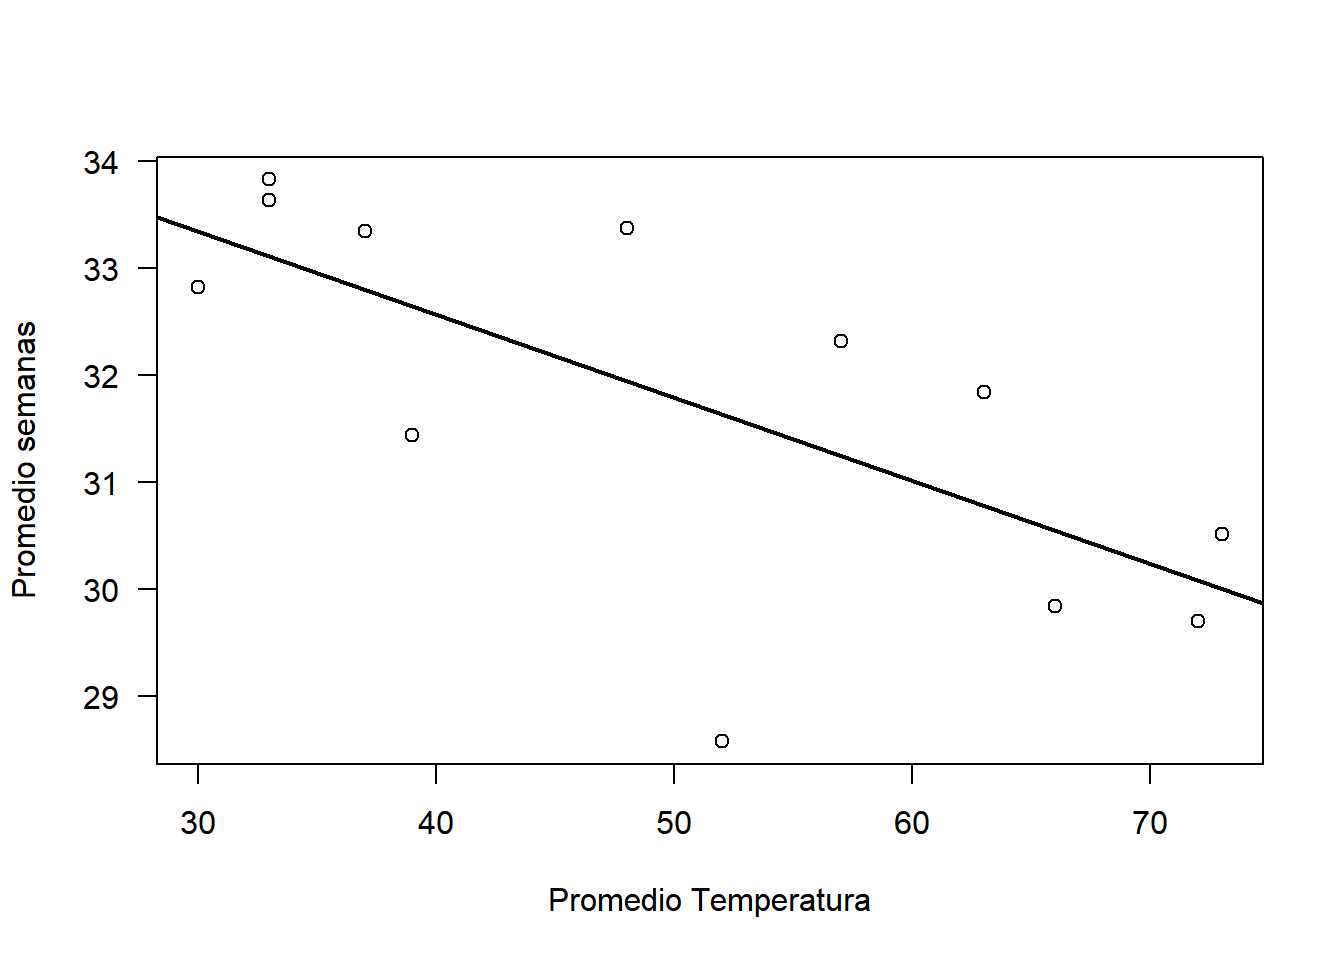
\includegraphics{Ejer_files/figure-latex/unnamed-chunk-2-1.pdf} Al
realizar la comparación del promedio de semanas hasta gatear y el
rpomedio de la temperatura en los siguientes 6 meses, se puede observar
una relativa linealidad decreciente, es decir, que en cuanto más frío
esté, menos son los reportes de que los niños gateen. Y se encuentra un
outlyer entre 50 y 60.

2.R\\

Porque la regresión ponderada se puede utilizar para corregir la
heterocedasticidad. En un procedimiento de regresión ponderada, se
otorga más peso a las observaciones con una varianza más pequeña porque
estas observaciones brindan información más confiable sobre la función
de regresión que aquellas con varianzas grandes. Observemos que la
varianza de las observaciones, asimismo la desviación estándar y un
histograma para ver si se ve normalidad.

Como son promedios y deben considerarse que los promedio son toamdos de
disntintas poblaciones.

\begin{Shaded}
\begin{Highlighting}[]
\CommentTok{\#var(Babies$PromedioTemperatura)}
\CommentTok{\#sd(Babies$PromedioTemperatura)}
\CommentTok{\#hist(Babies$PromedioTemperatura, breaks = 12)}
\end{Highlighting}
\end{Shaded}

3.R/

\begin{Shaded}
\begin{Highlighting}[]
\NormalTok{mod\_leo }\OtherTok{\textless{}{-}}  \FunctionTok{lm}\NormalTok{(PromedioSemanas }\SpecialCharTok{\textasciitilde{}}\NormalTok{ PromedioTemperatura, }\AttributeTok{data=}\NormalTok{Babies, }\AttributeTok{weights =}\NormalTok{ Frecuencia)}

\FunctionTok{coef}\NormalTok{(mod\_leo)}
\end{Highlighting}
\end{Shaded}

\begin{verbatim}
##         (Intercept) PromedioTemperatura 
##         35.70253928         -0.07560731
\end{verbatim}

Un aumento en una unidad de temperatura, que es unica covariable y
provoca una disminucuion de mas 0.75 en promedio en la edad promedio de
gateo, amnteniendo las demás variables constante. Un unidad de la
tempratura sube, indica que el promedio de la edad promedio baja en
o.075, nomina lmente, funcio de enlacio que es la identidad. Un aumento
de la temperatura proboca una disminucion de apro de 0.075 en promedio
de la edad promedio, como estamps viedno la esperanza, que estamos
viendo mu, que es la esperanza de Y.

Es importante ver que al menos sale negativo el coeficiente, que es lo
que espera el estudio,puesto que tienen una relación negativa.

\begin{enumerate}
\def\labelenumi{\arabic{enumi}.}
\setcounter{enumi}{3}
\tightlist
\item
  R/
\end{enumerate}

\begin{Shaded}
\begin{Highlighting}[]
\FunctionTok{summary}\NormalTok{(mod\_leo)}
\end{Highlighting}
\end{Shaded}

\begin{verbatim}
## 
## Call:
## lm(formula = PromedioSemanas ~ PromedioTemperatura, data = Babies, 
##     weights = Frecuencia)
## 
## Weighted Residuals:
##     Min      1Q  Median      3Q     Max 
## -16.581  -4.325   2.001   4.026   9.146 
## 
## Coefficients:
##                     Estimate Std. Error t value Pr(>|t|)    
## (Intercept)         35.70254    1.26003  28.335 6.97e-11 ***
## PromedioTemperatura -0.07561    0.02454  -3.081   0.0116 *  
## ---
## Signif. codes:  0 '***' 0.001 '**' 0.01 '*' 0.05 '.' 0.1 ' ' 1
## 
## Residual standard error: 7.399 on 10 degrees of freedom
## Multiple R-squared:  0.487,  Adjusted R-squared:  0.4357 
## F-statistic: 9.494 on 1 and 10 DF,  p-value: 0.01162
\end{verbatim}

Nos salio una prueba de t, con un nivel de 5\% de confianza, si se
rechaza y con un 1\% de significancia, no se rechaza.

5.R/

El IC95\% aporta al lector la precisión estadística. Por «precisión
estadística», se refiere a la incertidumbre introducida por los métodos
de muestreo. Es un intervalo bastante pequeño, lo cual sin ser muy
conservadores, se encuentra el rango de error. Esto es que el 90\% de
las veces, casi seguramente, el coeficiente de la varaible se va a
encontrar en ese intervalo.

\begin{Shaded}
\begin{Highlighting}[]
\FunctionTok{confint}\NormalTok{(mod\_leo, }\AttributeTok{level =} \FloatTok{0.9}\NormalTok{)}
\end{Highlighting}
\end{Shaded}

\begin{verbatim}
##                            5 %        95 %
## (Intercept)         33.4187757 37.98630282
## PromedioTemperatura -0.1200823 -0.03113231
\end{verbatim}

6.R/

\begin{Shaded}
\begin{Highlighting}[]
\NormalTok{mod\_leo2 }\OtherTok{\textless{}{-}}  \FunctionTok{lm}\NormalTok{(PromedioSemanas }\SpecialCharTok{\textasciitilde{}}\NormalTok{ PromedioTemperatura, }\AttributeTok{data=}\NormalTok{Babies)}

\FunctionTok{coef}\NormalTok{(mod\_leo)}
\end{Highlighting}
\end{Shaded}

\begin{verbatim}
##         (Intercept) PromedioTemperatura 
##         35.70253928         -0.07560731
\end{verbatim}

Un aumento en una unidad de temperatura, que es unica covariable y
provoca una disminucuion de mas 0.75 en promedio en la edad promedio de
gateo, amnteniendo las demás variables constante. Un unidad de la
tempratura sube, indica que el promedio de la edad promedio baja en
0.077, nomina lmente, funcio de enlacio que es la identidad. Un aumento
de la temperatura proboca una disminucion de apro de 0.077 en promedio
de la edad promedio, como estamps viedno la esperanza, que estamos
viendo mu, que es la esperanza de Y.

Es importante ver que al menos sale negativo el coeficiente, que es lo
que espera el estudio,puesto que tienen una relación negativa.

Entonces baja un 0.002, o sea el impacto es mayor.

\begin{Shaded}
\begin{Highlighting}[]
\FunctionTok{plot}\NormalTok{( PromedioSemanas }\SpecialCharTok{\textasciitilde{}}\NormalTok{ PromedioTemperatura, }\AttributeTok{data=}\NormalTok{Babies, }\AttributeTok{las=}\DecValTok{1}\NormalTok{,}
\AttributeTok{xlab=}\StringTok{"Promedio Temperatura"}\NormalTok{, }\AttributeTok{ylab=}\StringTok{"Promedio semanas"}\NormalTok{ )}
\FunctionTok{abline}\NormalTok{( }\FunctionTok{coef}\NormalTok{(p),}\AttributeTok{col=}\StringTok{"red"}\NormalTok{, }\AttributeTok{lty=}\DecValTok{1}\NormalTok{, }\AttributeTok{lwd=}\DecValTok{2}\NormalTok{)}
\FunctionTok{abline}\NormalTok{( }\FunctionTok{coef}\NormalTok{(mod\_leo),}\AttributeTok{col=}\StringTok{"blue"}\NormalTok{, }\AttributeTok{lty=}\DecValTok{1}\NormalTok{, }\AttributeTok{lwd=}\DecValTok{2}\NormalTok{)}
\end{Highlighting}
\end{Shaded}

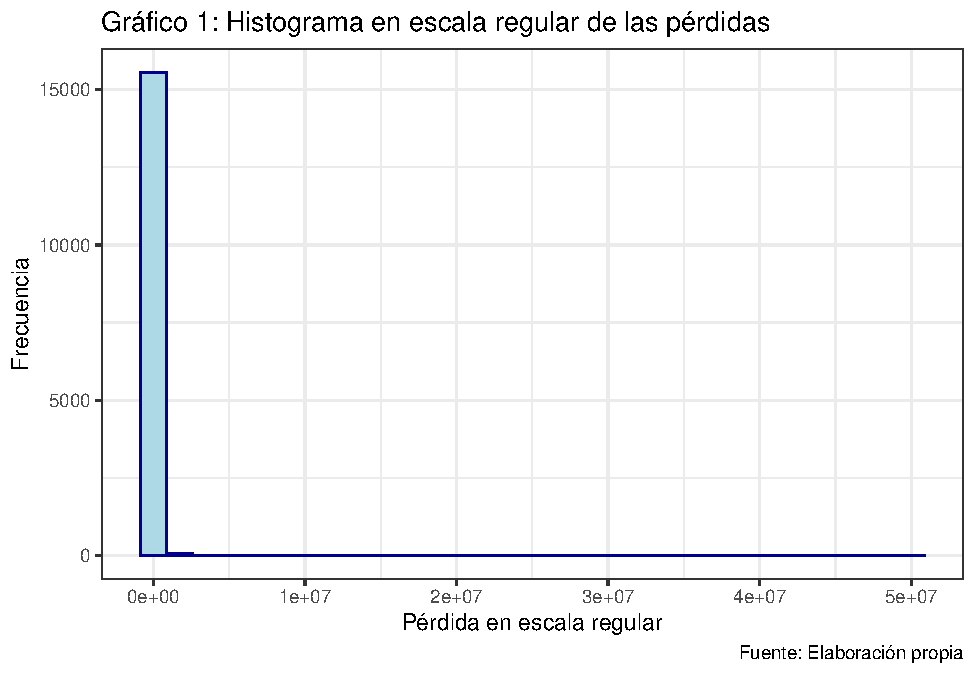
\includegraphics{Ejer_files/figure-latex/unnamed-chunk-8-1.pdf}

Asimismo, se puede ver mediante el gráfico una diferencia no tan
abismal.

7.R/

\begin{Shaded}
\begin{Highlighting}[]
\NormalTok{x}\OtherTok{\textless{}{-}}\NormalTok{Babies}\SpecialCharTok{$}\NormalTok{PromedioTemperatura}
\NormalTok{x }\OtherTok{\textless{}{-}}\NormalTok{(}\AttributeTok{PromedioTemperatura =} \FunctionTok{seq}\NormalTok{(}\FunctionTok{min}\NormalTok{(x), }\FunctionTok{max}\NormalTok{(x), }\AttributeTok{by =} \FloatTok{0.05}\NormalTok{))}
\NormalTok{cosa }\OtherTok{\textless{}{-}}
  \FunctionTok{predict}\NormalTok{(mod\_leo,}
          \AttributeTok{newdata =} \FunctionTok{data.frame}\NormalTok{(x),}
          \AttributeTok{interval =} \StringTok{"confidence"}\NormalTok{,}
          \AttributeTok{level =} \FloatTok{0.95}\NormalTok{)}


\FunctionTok{plot}\NormalTok{( PromedioSemanas }\SpecialCharTok{\textasciitilde{}}\NormalTok{ PromedioTemperatura, }\AttributeTok{data=}\NormalTok{Babies,}
      \AttributeTok{xlab =} \StringTok{"Promedio Temperatura"}\NormalTok{, }\AttributeTok{ylab =} \StringTok{"Promedio semanas"}\NormalTok{)}
\FunctionTok{abline}\NormalTok{(}\FunctionTok{coef}\NormalTok{(mod\_leo), }\AttributeTok{lty =} \DecValTok{1}\NormalTok{, }\AttributeTok{lwd =} \DecValTok{2}\NormalTok{)}
\FunctionTok{lines}\NormalTok{(x, cosa[,}\DecValTok{2}\NormalTok{], }\AttributeTok{col=}\StringTok{"blue"}\NormalTok{, }\AttributeTok{lty=}\DecValTok{2}\NormalTok{)}
\FunctionTok{lines}\NormalTok{(x, cosa[,}\DecValTok{3}\NormalTok{], }\AttributeTok{col=}\StringTok{"blue"}\NormalTok{, }\AttributeTok{lty=}\DecValTok{2}\NormalTok{)}
\end{Highlighting}
\end{Shaded}

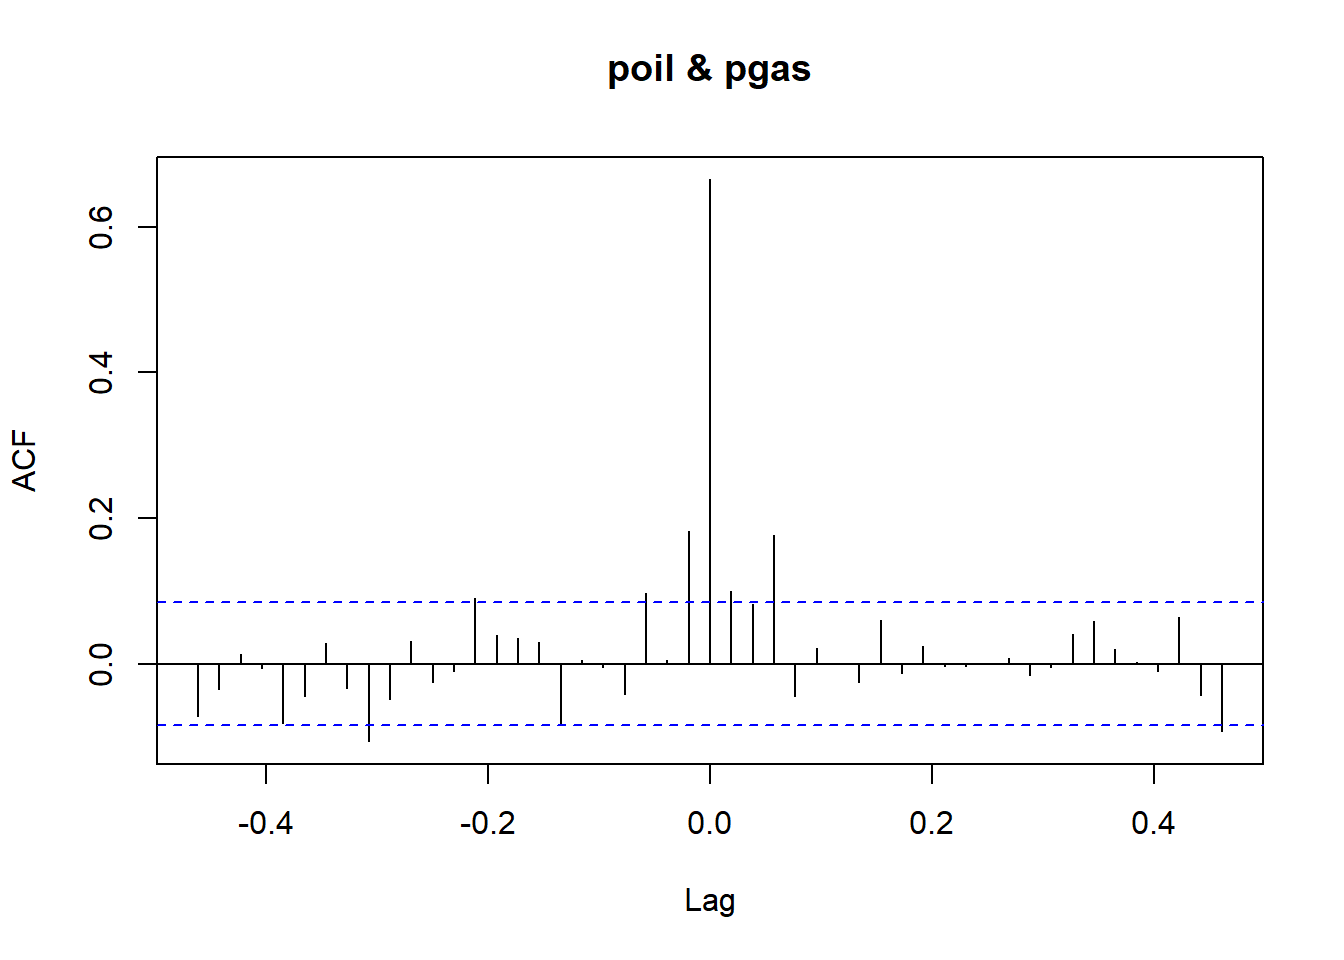
\includegraphics{Ejer_files/figure-latex/unnamed-chunk-9-1.pdf}

\begin{Shaded}
\begin{Highlighting}[]
\FunctionTok{library}\NormalTok{(ggplot2)}
\end{Highlighting}
\end{Shaded}

\begin{verbatim}
## Warning: package 'ggplot2' was built under R version 4.1.3
\end{verbatim}

\begin{Shaded}
\begin{Highlighting}[]
\FunctionTok{ggplot}\NormalTok{(}\AttributeTok{data =}\NormalTok{ Babies, }\AttributeTok{mapping =} \FunctionTok{aes}\NormalTok{(}\AttributeTok{x =}\NormalTok{ Babies}\SpecialCharTok{$}\NormalTok{PromedioTemperatura, }\AttributeTok{y =}\NormalTok{ Babies}\SpecialCharTok{$}\NormalTok{PromedioSemanas)) }\SpecialCharTok{+} \FunctionTok{geom\_point}\NormalTok{() }\SpecialCharTok{+} \FunctionTok{geom\_smooth}\NormalTok{(}\AttributeTok{method =}\NormalTok{ lm)}
\end{Highlighting}
\end{Shaded}

\begin{verbatim}
## Warning: Use of `Babies$PromedioTemperatura` is discouraged. Use
## `PromedioTemperatura` instead.
\end{verbatim}

\begin{verbatim}
## Warning: Use of `Babies$PromedioSemanas` is discouraged. Use `PromedioSemanas`
## instead.
\end{verbatim}

\begin{verbatim}
## Warning: Use of `Babies$PromedioTemperatura` is discouraged. Use
## `PromedioTemperatura` instead.
\end{verbatim}

\begin{verbatim}
## Warning: Use of `Babies$PromedioSemanas` is discouraged. Use `PromedioSemanas`
## instead.
\end{verbatim}

\begin{verbatim}
## `geom_smooth()` using formula 'y ~ x'
\end{verbatim}

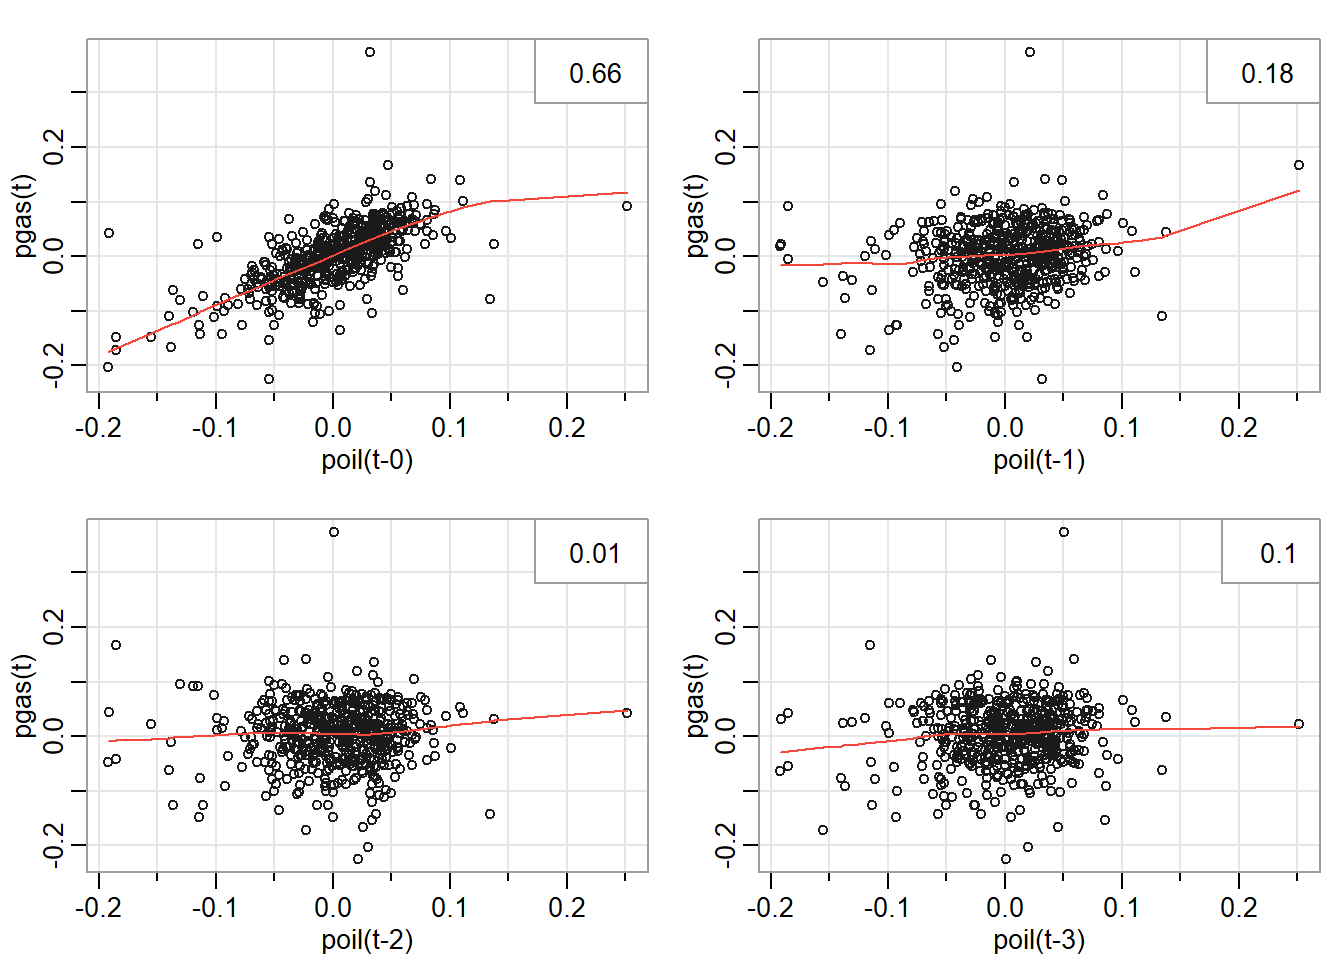
\includegraphics{Ejer_files/figure-latex/unnamed-chunk-10-1.pdf}

No reduce muy significativamente el intervalo de confianza, siendo un
5\% más conservadores, esto probablemente por la variabilidad de las
observaciones

\begin{Shaded}
\begin{Highlighting}[]
\FunctionTok{confint}\NormalTok{(mod\_leo, }\AttributeTok{level =} \FloatTok{0.95}\NormalTok{)}
\end{Highlighting}
\end{Shaded}

\begin{verbatim}
##                          2.5 %      97.5 %
## (Intercept)         32.8950075 38.51007110
## PromedioTemperatura -0.1302824 -0.02093222
\end{verbatim}

\begin{Shaded}
\begin{Highlighting}[]
\CommentTok{\#x \textless{}{-} Babies$PromedioTemperatura}
\CommentTok{\#x \textless{}{-}(PromedioTemperatura = seq(min(x), max(x), by = 0.05))}
\CommentTok{\#cosa \textless{}{-}}
\CommentTok{\#   predict(q,}
\CommentTok{\#           newdata = data.frame(x),}
\CommentTok{\#           interval = "confidence",}
\CommentTok{\#           level = 0.95)}
\CommentTok{\# }
\CommentTok{\# }
\CommentTok{\# plot( PromedioSemanas \textasciitilde{} PromedioTemperatura, data=Babies,}
\CommentTok{\#       xlab = "Promedio Temperatura", ylab = "Promedio semanas")}
\CommentTok{\# abline(coef(q), lty = 1, lwd = 2)}
\CommentTok{\# lines(x, cosa[,2], col="blue", lty=2)}
\CommentTok{\# lines(x, cosa[,3], col="blue", lty=2)}
\end{Highlighting}
\end{Shaded}

8.R/

Como rompe con el supuesto de variabilidad nula, entonces se necesita un
ajuste mediante los pesos, el cual no mejora significativamente la
regresión, lo importante es notar es que si se logra la relación inversa
con lo propuesto mediante la hip nula.

3.15. Un estudio de bebés {[}4{]} planteó la hipótesis de que los bebés
tardarían más en aprender a gatear en los meses más fríos porque la ropa
extra restringe su movimiento (conjunto de datos: rastreo). Los datos y
una descripción más completa se dan en Problema 2.16 (pág. 87). En ese
problema, se ajustó un modelo de regresión lineal a los datos 1. Realice
un análisis de diagnóstico del modelo de regresión lineal ajustado. 2.
Identifique las observaciones influyentes o los valores atípicos. 3.
Suponga que algunos de los bebés fueran mellizos. ¿Qué suposición sería
violado por la inclusión de estos bebés en el estudio? ¿Crees que esto
tendría implicaciones prácticas

1.R/

\begin{Shaded}
\begin{Highlighting}[]
\FunctionTok{rstandard}\NormalTok{(mod\_leo)}\CommentTok{\#residual estandarizado}
\end{Highlighting}
\end{Shaded}

\begin{verbatim}
##          1          2          3          4          5          6          7 
## -0.7352459  0.3292230 -0.4017996  0.6607410 -2.3206258 -1.0096045  0.2840962 
##          8          9         10         11         12 
## -0.6611690  0.5801706  0.4399001  1.3169833  0.8940981
\end{verbatim}

\begin{Shaded}
\begin{Highlighting}[]
\FunctionTok{fitted}\NormalTok{(mod\_leo) }\CommentTok{\#Este ejemplo demuestra cómo encontrar los valores ajustados de un modelo de regresión lineal usando la función added().}
\end{Highlighting}
\end{Shaded}

\begin{verbatim}
##        1        2        3        4        5        6        7        8 
## 30.71246 30.18321 30.25881 30.93928 31.77096 32.75385 33.20750 33.43432 
##        9       10       11       12 
## 33.20750 32.90507 32.07339 31.39292
\end{verbatim}

\begin{Shaded}
\begin{Highlighting}[]
\FunctionTok{cooks.distance}\NormalTok{(mod\_leo) }\CommentTok{\#La distancia de Cook es un resumen de cuánto cambia un modelo de regresión cuando se elimina la i{-}ésima observación}
\end{Highlighting}
\end{Shaded}

\begin{verbatim}
##           1           2           3           4           5           6 
## 0.058148988 0.024563962 0.018623041 0.029074790 0.195236233 0.058520287 
##           7           8           9          10          11          12 
## 0.005042211 0.089473010 0.042332772 0.020935096 0.117237279 0.062911737
\end{verbatim}

\begin{Shaded}
\begin{Highlighting}[]
 \FunctionTok{scatter.smooth}\NormalTok{( }\FunctionTok{rstandard}\NormalTok{(mod\_leo) }\SpecialCharTok{\textasciitilde{}} \FunctionTok{fitted}\NormalTok{(mod\_leo) )}
\end{Highlighting}
\end{Shaded}

\includegraphics{Ejer_files/figure-latex/unnamed-chunk-13-1.pdf}

\begin{Shaded}
\begin{Highlighting}[]
 \FunctionTok{qqnorm}\NormalTok{( }\FunctionTok{rstandard}\NormalTok{(mod\_leo) )}
 \FunctionTok{qqline}\NormalTok{( }\FunctionTok{rstandard}\NormalTok{(mod\_leo) )}
\end{Highlighting}
\end{Shaded}

\includegraphics{Ejer_files/figure-latex/unnamed-chunk-13-2.pdf}

\begin{Shaded}
\begin{Highlighting}[]
 \FunctionTok{plot}\NormalTok{( }\FunctionTok{cooks.distance}\NormalTok{(mod\_leo), }\AttributeTok{type=}\StringTok{"h"}\NormalTok{)}
\end{Highlighting}
\end{Shaded}

\includegraphics{Ejer_files/figure-latex/unnamed-chunk-13-3.pdf}

\begin{Shaded}
\begin{Highlighting}[]
 \FunctionTok{plot}\NormalTok{( }\FunctionTok{rstandard}\NormalTok{(mod\_leo) }\SpecialCharTok{\textasciitilde{}}\NormalTok{ Babies}\SpecialCharTok{$}\NormalTok{PromedioTemperatura)}
\end{Highlighting}
\end{Shaded}

\includegraphics{Ejer_files/figure-latex/unnamed-chunk-13-4.pdf}

2.R/

\begin{Shaded}
\begin{Highlighting}[]
\FunctionTok{influence.measures}\NormalTok{(mod\_leo)}\SpecialCharTok{$}\NormalTok{is.inf}
\end{Highlighting}
\end{Shaded}

\begin{verbatim}
##    dfb.1_ dfb.PrmT dffit cov.r cook.d   hat
## 1   FALSE    FALSE FALSE FALSE  FALSE FALSE
## 2   FALSE    FALSE FALSE  TRUE  FALSE FALSE
## 3   FALSE    FALSE FALSE FALSE  FALSE FALSE
## 4   FALSE    FALSE FALSE FALSE  FALSE FALSE
## 5   FALSE    FALSE FALSE  TRUE  FALSE FALSE
## 6   FALSE    FALSE FALSE FALSE  FALSE FALSE
## 7   FALSE    FALSE FALSE FALSE  FALSE FALSE
## 8   FALSE    FALSE FALSE FALSE  FALSE FALSE
## 9   FALSE    FALSE FALSE FALSE  FALSE FALSE
## 10  FALSE    FALSE FALSE FALSE  FALSE FALSE
## 11  FALSE    FALSE FALSE FALSE  FALSE FALSE
## 12  FALSE    FALSE FALSE FALSE  FALSE FALSE
\end{verbatim}

\begin{Shaded}
\begin{Highlighting}[]
\FunctionTok{rowSums}\NormalTok{(}\FunctionTok{influence.measures}\NormalTok{(mod\_leo)}\SpecialCharTok{$}\NormalTok{is.inf)}
\end{Highlighting}
\end{Shaded}

\begin{verbatim}
##  1  2  3  4  5  6  7  8  9 10 11 12 
##  0  1  0  0  1  0  0  0  0  0  0  0
\end{verbatim}

Hay una tendencia lineal, hay presencia de 3 outliers, el de la posición
2, 3 y 5, o se en febrero, marzo y mayo. Son de influencia.

3.R/

ausencia de outliers todas las fespuestas fiueron generadas por el mismo
proceso, de manera que el modelo de regresion es aporpiado para todas
las observaciones. Si hay outliers que sean obtenidos por el mismo
proceso de recopilacion de datos linealidad: El predictor lineal captura
la evrdadera relacion enrre mu\_i y las variables explicatoroas, todas
las variavles explicatorias importantes se incluyen varianza constante:
la variable respiesta yi tiene varianza constante, demás de pesos
conocidos como wi independencia: Def de independiente distribución: LA
variable respuesta está normalmente distribuida al rededor de su media
mui

R/Si hay gemelos, se rompe la de independencia.

5.25. Se pidió a los niños que construyeran torres tan altas como
pudieran a partir de cubos y bloques cilíndricos {[}2, 9{]}. El número
de bloques utilizados y el tiempo empleado fueron registrados (Tabla
2.12; conjunto de datos: bloques). En este problema, sólo considere el
número de bloques utilizados y y la edad del niño x.

\begin{enumerate}
\def\labelenumi{\arabic{enumi}.}
\item
  Grafique el número de bloques usados contra la edad del niño.
\item
  A partir de la gráfica y la comprensión de los datos, responda las dos
  preguntas para estos datos y, por lo tanto, proponga un glm para los
  datos.
\end{enumerate}

1.R/

\begin{Shaded}
\begin{Highlighting}[]
\FunctionTok{library}\NormalTok{(}\StringTok{"GLMsData"}\NormalTok{) }
\FunctionTok{data}\NormalTok{(blocks)}

 \CommentTok{\#par(mfrow=c(1, 2))}
 \CommentTok{\#plot(jitter(Number)\textasciitilde{}Age, data=blocks)}
 \CommentTok{\#plot( Number\textasciitilde{}cut(Age, 3), data=blocks)}
\FunctionTok{plot}\NormalTok{( }\FunctionTok{jitter}\NormalTok{(Number)}\SpecialCharTok{\textasciitilde{}}\NormalTok{Age,  }\AttributeTok{data=}\NormalTok{blocks, }\AttributeTok{las=}\DecValTok{1}\NormalTok{,}
\AttributeTok{xlab=}\StringTok{"Número de bloques"}\NormalTok{, }\AttributeTok{ylab=}\StringTok{"Edad del niño"}\NormalTok{ ) }\CommentTok{\#el jitter agrega un poco de ruido, para que se traslap}
\end{Highlighting}
\end{Shaded}

\includegraphics{Ejer_files/figure-latex/unnamed-chunk-15-1.pdf} 1. ¿Qué
distribución de probabilidad es apropiada? La respuesta determina la
componente aleatoria del modelo. La elección de la distribución de
probabilidad pueden ser sugeridos por los datos de respuesta (por
ejemplo, proporciones de un total sugieren una distribución binomial), o
el conocimiento de cómo la varianza cambia con la media.

\begin{Shaded}
\begin{Highlighting}[]
\FunctionTok{var}\NormalTok{(blocks}\SpecialCharTok{$}\NormalTok{Number)}
\end{Highlighting}
\end{Shaded}

\begin{verbatim}
## [1] 4.977374
\end{verbatim}

\begin{Shaded}
\begin{Highlighting}[]
\FunctionTok{mean}\NormalTok{(blocks}\SpecialCharTok{$}\NormalTok{Number)}
\end{Highlighting}
\end{Shaded}

\begin{verbatim}
## [1] 6.82
\end{verbatim}

\begin{Shaded}
\begin{Highlighting}[]
\FunctionTok{sd}\NormalTok{((blocks}\SpecialCharTok{$}\NormalTok{Number))}
\end{Highlighting}
\end{Shaded}

\begin{verbatim}
## [1] 2.231003
\end{verbatim}

La varianza es menor a la esperanza(media), es una distribución poisson

\begin{enumerate}
\def\labelenumi{\arabic{enumi}.}
\setcounter{enumi}{1}
\tightlist
\item
  ¿Cómo se relacionan las variables explicativas con la media de la
  respuesta? ¿? La respuesta sugiere el componente sistemático del
  modelo. glms asumir una función que une el predictor lineal η = β0 + p
  j=1 βjxj a la media μ, como log μ = η por ejemplo. Es decir, glms son
  regresión modelos lineales en los parámetros.
\end{enumerate}

se relaciona de una manera similar

6.10. Se pidió a los niños que construyeran torres tan altas como
pudieran a partir de cubos y bloques cilíndricos {[}3, 6{]}. El número
de bloques utilizados y el tiempo empleado fueron registrados (conjunto
de datos: bloques). En este problema, sólo considere el número de
bloques utilizados y y la edad del niño x. En el Problema 5.25, un glm
fue propuesta para estos datos. 1. Ajuste este glm usando r y escriba el
modelo ajustado. 2. Determinar el error estándar para cada parámetro de
regresión. 3. Calcule la desviación residual.

1.R/

\begin{Shaded}
\begin{Highlighting}[]
\FunctionTok{data}\NormalTok{(blocks)}
\NormalTok{ m1 }\OtherTok{\textless{}{-}} \FunctionTok{glm}\NormalTok{(Number}\SpecialCharTok{\textasciitilde{}}\NormalTok{Age, }\AttributeTok{data=}\NormalTok{blocks, }\AttributeTok{family=}\NormalTok{poisson)}
\end{Highlighting}
\end{Shaded}

2.R/

\begin{Shaded}
\begin{Highlighting}[]
\FunctionTok{deviance}\NormalTok{(m1)}
\end{Highlighting}
\end{Shaded}

\begin{verbatim}
## [1] 62.24384
\end{verbatim}

3.R/

\begin{Shaded}
\begin{Highlighting}[]
\FunctionTok{summary}\NormalTok{(m1)}
\end{Highlighting}
\end{Shaded}

\begin{verbatim}
## 
## Call:
## glm(formula = Number ~ Age, family = poisson, data = blocks)
## 
## Deviance Residuals: 
##     Min       1Q   Median       3Q      Max  
## -1.4977  -0.6542  -0.1984   0.4714   1.8155  
## 
## Coefficients:
##             Estimate Std. Error z value Pr(>|z|)    
## (Intercept)   1.3447     0.2223   6.048 1.47e-09 ***
## Age           0.1415     0.0534   2.650  0.00805 ** 
## ---
## Signif. codes:  0 '***' 0.001 '**' 0.01 '*' 0.05 '.' 0.1 ' ' 1
## 
## (Dispersion parameter for poisson family taken to be 1)
## 
##     Null deviance: 69.429  on 99  degrees of freedom
## Residual deviance: 62.244  on 98  degrees of freedom
## AIC: 439.64
## 
## Number of Fisher Scoring iterations: 4
\end{verbatim}

\begin{Shaded}
\begin{Highlighting}[]
\NormalTok{m1}\SpecialCharTok{$}\NormalTok{null.deviance }\SpecialCharTok{{-}}\NormalTok{ m1}\SpecialCharTok{$}\NormalTok{deviance}
\end{Highlighting}
\end{Shaded}

\begin{verbatim}
## [1] 7.185388
\end{verbatim}

\begin{Shaded}
\begin{Highlighting}[]
\DecValTok{1} \SpecialCharTok{{-}} \FunctionTok{pchisq}\NormalTok{ (}\FloatTok{7.185388}\NormalTok{, }\DecValTok{1}\NormalTok{)}
\end{Highlighting}
\end{Shaded}

\begin{verbatim}
## [1] 0.007349966
\end{verbatim}

Se puede rechazar claramente la hipótesis nula. Hay una relación
significativa con la edad.

7.4. Se pidió a los niños que construyeran torres tan altas como
pudieran a partir de cubos y bloques cilíndricos {[}3, 7{]}. El número
de bloques utilizados y el tiempo empleado fueron registrados (conjunto
de datos: bloques). En este problema, sólo considere el número de
bloques utilizados y y la edad del niño x. En el problema 6.10, se
ajustó un glm para estos datos. 1. Use una prueba de Wald para
determinar si la edad parece necesaria en el modelo. 2. Use una prueba
de puntuación para determinar si la edad parece necesaria en el modelo.
3. Usar una prueba de razón de verosimilitud para determinar si la edad
parece necesaria en el modelo. 4. Compare los resultados de las pruebas
de Wald, puntuación y razón de verosimilitud. comentario. 5. ¿Se espera
que la aproximación del punto de silla sea precisa? Explique. 6. ¿Se
espera que el teorema del límite central sea exacto? Explique. 7. Halle
los intervalos de confianza de Wald al 95 \% para los coeficientes de
regresión. 8. Grafique el número de bloques usados contra la edad y
muestre la relación descrito por el modelo ajustado. Traza también las
rectas que indican el debajo y sobre al 95\% de IC para estos valores
ajustados.

\begin{Shaded}
\begin{Highlighting}[]
\FunctionTok{data}\NormalTok{(blocks); }\FunctionTok{library}\NormalTok{(statmod)}
\end{Highlighting}
\end{Shaded}

\begin{verbatim}
## Warning: package 'statmod' was built under R version 4.1.3
\end{verbatim}

\begin{Shaded}
\begin{Highlighting}[]
\NormalTok{ m1 }\OtherTok{\textless{}{-}} \FunctionTok{glm}\NormalTok{(Number}\SpecialCharTok{\textasciitilde{}}\NormalTok{Age, }\AttributeTok{data=}\NormalTok{blocks, }\AttributeTok{family=}\NormalTok{poisson)}
\NormalTok{ m0 }\OtherTok{\textless{}{-}} \FunctionTok{update}\NormalTok{(m1, .}\SpecialCharTok{\textasciitilde{}}\DecValTok{1}\NormalTok{)}
\end{Highlighting}
\end{Shaded}

1.R/

\begin{Shaded}
\begin{Highlighting}[]
\FunctionTok{summary}\NormalTok{(m1)}
\end{Highlighting}
\end{Shaded}

\begin{verbatim}
## 
## Call:
## glm(formula = Number ~ Age, family = poisson, data = blocks)
## 
## Deviance Residuals: 
##     Min       1Q   Median       3Q      Max  
## -1.4977  -0.6542  -0.1984   0.4714   1.8155  
## 
## Coefficients:
##             Estimate Std. Error z value Pr(>|z|)    
## (Intercept)   1.3447     0.2223   6.048 1.47e-09 ***
## Age           0.1415     0.0534   2.650  0.00805 ** 
## ---
## Signif. codes:  0 '***' 0.001 '**' 0.01 '*' 0.05 '.' 0.1 ' ' 1
## 
## (Dispersion parameter for poisson family taken to be 1)
## 
##     Null deviance: 69.429  on 99  degrees of freedom
## Residual deviance: 62.244  on 98  degrees of freedom
## AIC: 439.64
## 
## Number of Fisher Scoring iterations: 4
\end{verbatim}

\begin{Shaded}
\begin{Highlighting}[]
\NormalTok{(z.Wald }\OtherTok{\textless{}{-}} \FunctionTok{coef}\NormalTok{(}\FunctionTok{summary}\NormalTok{(m1))[}\DecValTok{2}\NormalTok{, }\DecValTok{3}\NormalTok{])}
\end{Highlighting}
\end{Shaded}

\begin{verbatim}
## [1] 2.649974
\end{verbatim}

\begin{Shaded}
\begin{Highlighting}[]
\NormalTok{ (P.Wald }\OtherTok{\textless{}{-}} \FunctionTok{coef}\NormalTok{(}\FunctionTok{summary}\NormalTok{(m1))[}\DecValTok{2}\NormalTok{, }\DecValTok{4}\NormalTok{])}
\end{Highlighting}
\end{Shaded}

\begin{verbatim}
## [1] 0.008049803
\end{verbatim}

La edad tiene una significancia de 0.001, estonces sí es necesaria

2.R/

\begin{Shaded}
\begin{Highlighting}[]
\NormalTok{( z.score }\OtherTok{\textless{}{-}} \FunctionTok{glm.scoretest}\NormalTok{(m0, blocks}\SpecialCharTok{$}\NormalTok{Age))}\CommentTok{\#Calcula las estadísticas de las pruebas de puntuación (estadísticas z) para agregar covariables a un modelo lineal generalizado.}
\end{Highlighting}
\end{Shaded}

\begin{verbatim}
## [1] 2.652281
\end{verbatim}

\begin{Shaded}
\begin{Highlighting}[]
\NormalTok{( P.score }\OtherTok{\textless{}{-}} \DecValTok{2}\SpecialCharTok{*}\NormalTok{(}\DecValTok{1}\SpecialCharTok{{-}}\FunctionTok{pt}\NormalTok{(}\FunctionTok{abs}\NormalTok{(z.score), }\AttributeTok{df=}\FunctionTok{df.residual}\NormalTok{(m1)))) }\CommentTok{\#La función pt devuelve el valor de la función de densidad acumulada (cdf) de la distribución t de Student dada una determinada variable aleatoria x y grados de libertad df}
\end{Highlighting}
\end{Shaded}

\begin{verbatim}
## [1] 0.009326481
\end{verbatim}

\begin{Shaded}
\begin{Highlighting}[]
\CommentTok{\#por ser t student y su simetría ent quedaría = 2(1 − Pr \{zscore \textless{} grados de libertad\}).}
\end{Highlighting}
\end{Shaded}

Pues con este modelo, se de muestras que es de significancia la edad

3.R/

\begin{Shaded}
\begin{Highlighting}[]
\FunctionTok{anova}\NormalTok{(m1)}
\end{Highlighting}
\end{Shaded}

\begin{verbatim}
## Analysis of Deviance Table
## 
## Model: poisson, link: log
## 
## Response: Number
## 
## Terms added sequentially (first to last)
## 
## 
##      Df Deviance Resid. Df Resid. Dev
## NULL                    99     69.429
## Age   1   7.1854        98     62.244
\end{verbatim}

\begin{Shaded}
\begin{Highlighting}[]
\FunctionTok{anova}\NormalTok{(m1, }\AttributeTok{test=}\StringTok{"Chisq"}\NormalTok{)}
\end{Highlighting}
\end{Shaded}

\begin{verbatim}
## Analysis of Deviance Table
## 
## Model: poisson, link: log
## 
## Response: Number
## 
## Terms added sequentially (first to last)
## 
## 
##      Df Deviance Resid. Df Resid. Dev Pr(>Chi)   
## NULL                    99     69.429            
## Age   1   7.1854        98     62.244  0.00735 **
## ---
## Signif. codes:  0 '***' 0.001 '**' 0.01 '*' 0.05 '.' 0.1 ' ' 1
\end{verbatim}

\begin{Shaded}
\begin{Highlighting}[]
\NormalTok{(chisq.LRT }\OtherTok{\textless{}{-}} \FunctionTok{anova}\NormalTok{(m1)[}\DecValTok{2}\NormalTok{, }\DecValTok{2}\NormalTok{])}
\end{Highlighting}
\end{Shaded}

\begin{verbatim}
## [1] 7.185388
\end{verbatim}

\begin{Shaded}
\begin{Highlighting}[]
\NormalTok{( P.LRT }\OtherTok{\textless{}{-}} \FunctionTok{anova}\NormalTok{(m1, }\AttributeTok{test=}\StringTok{"Chisq"}\NormalTok{)[}\DecValTok{2}\NormalTok{, }\DecValTok{5}\NormalTok{])}
\end{Highlighting}
\end{Shaded}

\begin{verbatim}
## [1] 0.007349966
\end{verbatim}

También se demuestra con un 0.001 la significancia de la edad con la
verosimilitud 4.R/

\begin{Shaded}
\begin{Highlighting}[]
 \FunctionTok{c}\NormalTok{(z.Wald, z.score, }\FunctionTok{sqrt}\NormalTok{(chisq.LRT))}
\end{Highlighting}
\end{Shaded}

\begin{verbatim}
## [1] 2.649974 2.652281 2.680557
\end{verbatim}

\begin{Shaded}
\begin{Highlighting}[]
 \FunctionTok{round}\NormalTok{(}\FunctionTok{c}\NormalTok{(P.Wald, P.score, P.LRT), }\DecValTok{4}\NormalTok{)}
\end{Highlighting}
\end{Shaded}

\begin{verbatim}
## [1] 0.0080 0.0093 0.0073
\end{verbatim}

Se puede observar que con la prueba de likehood, pues la significancia
de la edad es la más cercana a 0, o sea la que más ve relevante la edad

5.R/ Para un glm de Poisson, se espera que la aproximación del punto de
silla sea suficiente si el menor y ≥ 3; aquí el mínimo es 3, así que se
espera que la aproximación del punto de silla esté bien.

\begin{Shaded}
\begin{Highlighting}[]
\FunctionTok{min}\NormalTok{(blocks}\SpecialCharTok{$}\NormalTok{Number)}
\end{Highlighting}
\end{Shaded}

\begin{verbatim}
## [1] 3
\end{verbatim}

6.R/Para un glm de Poisson, se espera que la aproximación teorema del
limite central sea suficiente si es y ≥ 5; aquí el mínimo es 3, por lo
que la aproximación teorema del limite central puede ser
insuficientemente preciso.

7.R/

\begin{Shaded}
\begin{Highlighting}[]
\FunctionTok{confint}\NormalTok{(m1)}
\end{Highlighting}
\end{Shaded}

\begin{verbatim}
## Waiting for profiling to be done...
\end{verbatim}

\begin{verbatim}
##                 2.5 %    97.5 %
## (Intercept) 0.9024058 1.7742235
## Age         0.0377308 0.2471074
\end{verbatim}

8.R/

\begin{Shaded}
\begin{Highlighting}[]
\NormalTok{ newA }\OtherTok{\textless{}{-}} \FunctionTok{seq}\NormalTok{( }\FunctionTok{min}\NormalTok{(blocks}\SpecialCharTok{$}\NormalTok{Age), }\FunctionTok{max}\NormalTok{(blocks}\SpecialCharTok{$}\NormalTok{Age), }\AttributeTok{length=}\DecValTok{100}\NormalTok{)}
\NormalTok{ newB }\OtherTok{\textless{}{-}} \FunctionTok{predict}\NormalTok{( m1, }\AttributeTok{newdata=}\FunctionTok{data.frame}\NormalTok{(}\AttributeTok{Age=}\NormalTok{newA), }\AttributeTok{type=}\StringTok{"response"}\NormalTok{,}
\AttributeTok{se.fit=}\ConstantTok{TRUE}\NormalTok{)}
\FunctionTok{plot}\NormalTok{( }\FunctionTok{jitter}\NormalTok{(Number)}\SpecialCharTok{\textasciitilde{}}\NormalTok{Age, }\AttributeTok{data=}\NormalTok{blocks)}
 \FunctionTok{lines}\NormalTok{(newB}\SpecialCharTok{$}\NormalTok{fit }\SpecialCharTok{\textasciitilde{}}\NormalTok{ newA, }\AttributeTok{lwd=}\DecValTok{2}\NormalTok{)}
\NormalTok{ t.star }\OtherTok{\textless{}{-}} \FunctionTok{qt}\NormalTok{(}\AttributeTok{p=}\FloatTok{0.975}\NormalTok{, }\AttributeTok{df=}\FunctionTok{df.residual}\NormalTok{(m1))}
\NormalTok{ ci.lo }\OtherTok{\textless{}{-}}\NormalTok{ newB}\SpecialCharTok{$}\NormalTok{fit }\SpecialCharTok{{-}}\NormalTok{ t.star }\SpecialCharTok{*}\NormalTok{ newB}\SpecialCharTok{$}\NormalTok{se.fit}
\NormalTok{ ci.hi }\OtherTok{\textless{}{-}}\NormalTok{ newB}\SpecialCharTok{$}\NormalTok{fit }\SpecialCharTok{+}\NormalTok{ t.star }\SpecialCharTok{*}\NormalTok{ newB}\SpecialCharTok{$}\NormalTok{se.fit}
 \FunctionTok{lines}\NormalTok{(ci.lo}\SpecialCharTok{\textasciitilde{}}\NormalTok{newA, }\AttributeTok{lty=}\DecValTok{2}\NormalTok{)}
 \FunctionTok{lines}\NormalTok{(ci.hi}\SpecialCharTok{\textasciitilde{}}\NormalTok{newA, }\AttributeTok{lty=}\DecValTok{2}\NormalTok{)}
\end{Highlighting}
\end{Shaded}

\includegraphics{Ejer_files/figure-latex/unnamed-chunk-28-1.pdf}

8.11. Se pidió a los niños que construyeran torres tan altas como
pudieran a partir de cubos y bloques cilíndricos {[}8, 14{]}. El número
de bloques utilizados y el tiempo empleado fueron registrados (conjunto
de datos: bloques). En este problema, sólo considere el número de
bloques utilizados y y la edad del niño x. En el problema 6.10, se
ajustó un glm para estos datos. Realizar un diagnóstico análisis y
determinar si el modelo es adecuado

\begin{Shaded}
\begin{Highlighting}[]
 \FunctionTok{data}\NormalTok{(blocks)}
\FunctionTok{library}\NormalTok{(statmod)}
\NormalTok{ m3 }\OtherTok{\textless{}{-}} \FunctionTok{glm}\NormalTok{(Number}\SpecialCharTok{\textasciitilde{}}\NormalTok{Age, }\AttributeTok{data=}\NormalTok{blocks, }\AttributeTok{family=}\NormalTok{poisson)}
 \FunctionTok{par}\NormalTok{(}\AttributeTok{mfrow=}\FunctionTok{c}\NormalTok{(}\DecValTok{2}\NormalTok{, }\DecValTok{2}\NormalTok{))}
 \FunctionTok{plot}\NormalTok{( }\FunctionTok{rstandard}\NormalTok{(m3)}\SpecialCharTok{\textasciitilde{}}\FunctionTok{fitted}\NormalTok{(m3))}
 \FunctionTok{plot}\NormalTok{(}\FunctionTok{cooks.distance}\NormalTok{(m3), }\AttributeTok{type=}\StringTok{"h"}\NormalTok{)}
 \FunctionTok{qqnorm}\NormalTok{(}\FunctionTok{rstandard}\NormalTok{(m3))}
 \FunctionTok{qqnorm}\NormalTok{(}\FunctionTok{qresid}\NormalTok{(m3))}
\end{Highlighting}
\end{Shaded}

\includegraphics{Ejer_files/figure-latex/unnamed-chunk-29-1.pdf}

\begin{Shaded}
\begin{Highlighting}[]
 \FunctionTok{colSums}\NormalTok{(}\FunctionTok{influence.measures}\NormalTok{(m3)}\SpecialCharTok{$}\NormalTok{is.inf)}
\end{Highlighting}
\end{Shaded}

\begin{verbatim}
##  dfb.1_ dfb.Age   dffit   cov.r  cook.d     hat 
##       0       0       0       7       0       0
\end{verbatim}

\begin{Shaded}
\begin{Highlighting}[]
 \FunctionTok{influence.measures}\NormalTok{(m3)}\SpecialCharTok{$}\NormalTok{is.inf}
\end{Highlighting}
\end{Shaded}

\begin{verbatim}
##     dfb.1_ dfb.Age dffit cov.r cook.d   hat
## 1    FALSE   FALSE FALSE FALSE  FALSE FALSE
## 2    FALSE   FALSE FALSE FALSE  FALSE FALSE
## 3    FALSE   FALSE FALSE FALSE  FALSE FALSE
## 4    FALSE   FALSE FALSE FALSE  FALSE FALSE
## 5    FALSE   FALSE FALSE FALSE  FALSE FALSE
## 6    FALSE   FALSE FALSE FALSE  FALSE FALSE
## 7    FALSE   FALSE FALSE FALSE  FALSE FALSE
## 8    FALSE   FALSE FALSE FALSE  FALSE FALSE
## 9    FALSE   FALSE FALSE FALSE  FALSE FALSE
## 10   FALSE   FALSE FALSE  TRUE  FALSE FALSE
## 11   FALSE   FALSE FALSE FALSE  FALSE FALSE
## 12   FALSE   FALSE FALSE FALSE  FALSE FALSE
## 13   FALSE   FALSE FALSE FALSE  FALSE FALSE
## 14   FALSE   FALSE FALSE FALSE  FALSE FALSE
## 15   FALSE   FALSE FALSE FALSE  FALSE FALSE
## 16   FALSE   FALSE FALSE FALSE  FALSE FALSE
## 17   FALSE   FALSE FALSE FALSE  FALSE FALSE
## 18   FALSE   FALSE FALSE FALSE  FALSE FALSE
## 19   FALSE   FALSE FALSE FALSE  FALSE FALSE
## 20   FALSE   FALSE FALSE FALSE  FALSE FALSE
## 21   FALSE   FALSE FALSE FALSE  FALSE FALSE
## 22   FALSE   FALSE FALSE  TRUE  FALSE FALSE
## 23   FALSE   FALSE FALSE FALSE  FALSE FALSE
## 24   FALSE   FALSE FALSE FALSE  FALSE FALSE
## 25   FALSE   FALSE FALSE FALSE  FALSE FALSE
## 26   FALSE   FALSE FALSE FALSE  FALSE FALSE
## 27   FALSE   FALSE FALSE FALSE  FALSE FALSE
## 28   FALSE   FALSE FALSE FALSE  FALSE FALSE
## 29   FALSE   FALSE FALSE FALSE  FALSE FALSE
## 30   FALSE   FALSE FALSE FALSE  FALSE FALSE
## 31   FALSE   FALSE FALSE FALSE  FALSE FALSE
## 32   FALSE   FALSE FALSE FALSE  FALSE FALSE
## 33   FALSE   FALSE FALSE FALSE  FALSE FALSE
## 34   FALSE   FALSE FALSE FALSE  FALSE FALSE
## 35   FALSE   FALSE FALSE FALSE  FALSE FALSE
## 36   FALSE   FALSE FALSE FALSE  FALSE FALSE
## 37   FALSE   FALSE FALSE FALSE  FALSE FALSE
## 38   FALSE   FALSE FALSE FALSE  FALSE FALSE
## 39   FALSE   FALSE FALSE FALSE  FALSE FALSE
## 40   FALSE   FALSE FALSE FALSE  FALSE FALSE
## 41   FALSE   FALSE FALSE FALSE  FALSE FALSE
## 42   FALSE   FALSE FALSE FALSE  FALSE FALSE
## 43   FALSE   FALSE FALSE FALSE  FALSE FALSE
## 44   FALSE   FALSE FALSE  TRUE  FALSE FALSE
## 45   FALSE   FALSE FALSE FALSE  FALSE FALSE
## 46   FALSE   FALSE FALSE FALSE  FALSE FALSE
## 47   FALSE   FALSE FALSE FALSE  FALSE FALSE
## 48   FALSE   FALSE FALSE FALSE  FALSE FALSE
## 49   FALSE   FALSE FALSE FALSE  FALSE FALSE
## 50   FALSE   FALSE FALSE FALSE  FALSE FALSE
## 51   FALSE   FALSE FALSE FALSE  FALSE FALSE
## 52   FALSE   FALSE FALSE FALSE  FALSE FALSE
## 53   FALSE   FALSE FALSE FALSE  FALSE FALSE
## 54   FALSE   FALSE FALSE FALSE  FALSE FALSE
## 55   FALSE   FALSE FALSE FALSE  FALSE FALSE
## 56   FALSE   FALSE FALSE FALSE  FALSE FALSE
## 57   FALSE   FALSE FALSE FALSE  FALSE FALSE
## 58   FALSE   FALSE FALSE FALSE  FALSE FALSE
## 59   FALSE   FALSE FALSE FALSE  FALSE FALSE
## 60   FALSE   FALSE FALSE FALSE  FALSE FALSE
## 61   FALSE   FALSE FALSE FALSE  FALSE FALSE
## 62   FALSE   FALSE FALSE FALSE  FALSE FALSE
## 63   FALSE   FALSE FALSE FALSE  FALSE FALSE
## 64   FALSE   FALSE FALSE FALSE  FALSE FALSE
## 65   FALSE   FALSE FALSE FALSE  FALSE FALSE
## 66   FALSE   FALSE FALSE FALSE  FALSE FALSE
## 67   FALSE   FALSE FALSE FALSE  FALSE FALSE
## 68   FALSE   FALSE FALSE FALSE  FALSE FALSE
## 69   FALSE   FALSE FALSE  TRUE  FALSE FALSE
## 70   FALSE   FALSE FALSE FALSE  FALSE FALSE
## 71   FALSE   FALSE FALSE FALSE  FALSE FALSE
## 72   FALSE   FALSE FALSE  TRUE  FALSE FALSE
## 73   FALSE   FALSE FALSE FALSE  FALSE FALSE
## 74   FALSE   FALSE FALSE FALSE  FALSE FALSE
## 75   FALSE   FALSE FALSE FALSE  FALSE FALSE
## 76   FALSE   FALSE FALSE FALSE  FALSE FALSE
## 77   FALSE   FALSE FALSE FALSE  FALSE FALSE
## 78   FALSE   FALSE FALSE FALSE  FALSE FALSE
## 79   FALSE   FALSE FALSE FALSE  FALSE FALSE
## 80   FALSE   FALSE FALSE FALSE  FALSE FALSE
## 81   FALSE   FALSE FALSE FALSE  FALSE FALSE
## 82   FALSE   FALSE FALSE FALSE  FALSE FALSE
## 83   FALSE   FALSE FALSE FALSE  FALSE FALSE
## 84   FALSE   FALSE FALSE FALSE  FALSE FALSE
## 85   FALSE   FALSE FALSE FALSE  FALSE FALSE
## 86   FALSE   FALSE FALSE FALSE  FALSE FALSE
## 87   FALSE   FALSE FALSE FALSE  FALSE FALSE
## 88   FALSE   FALSE FALSE FALSE  FALSE FALSE
## 89   FALSE   FALSE FALSE FALSE  FALSE FALSE
## 90   FALSE   FALSE FALSE FALSE  FALSE FALSE
## 91   FALSE   FALSE FALSE FALSE  FALSE FALSE
## 92   FALSE   FALSE FALSE FALSE  FALSE FALSE
## 93   FALSE   FALSE FALSE FALSE  FALSE FALSE
## 94   FALSE   FALSE FALSE  TRUE  FALSE FALSE
## 95   FALSE   FALSE FALSE  TRUE  FALSE FALSE
## 96   FALSE   FALSE FALSE FALSE  FALSE FALSE
## 97   FALSE   FALSE FALSE FALSE  FALSE FALSE
## 98   FALSE   FALSE FALSE FALSE  FALSE FALSE
## 99   FALSE   FALSE FALSE FALSE  FALSE FALSE
## 100  FALSE   FALSE FALSE FALSE  FALSE FALSE
\end{verbatim}

\begin{Shaded}
\begin{Highlighting}[]
\FunctionTok{which}\NormalTok{(}\FunctionTok{rowSums}\NormalTok{(}\FunctionTok{influence.measures}\NormalTok{(m3)}\SpecialCharTok{$}\NormalTok{is.inf)}\SpecialCharTok{\textgreater{}}\DecValTok{0}\NormalTok{)}
\end{Highlighting}
\end{Shaded}

\begin{verbatim}
## 10 22 44 69 72 94 95 
## 10 22 44 69 72 94 95
\end{verbatim}

\begin{Shaded}
\begin{Highlighting}[]
\FunctionTok{deviance}\NormalTok{(m3)}
\end{Highlighting}
\end{Shaded}

\begin{verbatim}
## [1] 62.24384
\end{verbatim}

\begin{Shaded}
\begin{Highlighting}[]
\FunctionTok{df.residual}\NormalTok{(m3)}
\end{Highlighting}
\end{Shaded}

\begin{verbatim}
## [1] 98
\end{verbatim}

Hay una tendencia lineal. Hay alta influencia en las observaciones 10 22
44 69 72 94 95, no s eve una alta variabilidad. Está mal ajustado,
puesto que su devianza es muy alta

9.10. El periódico Independent tabuló el género de todos los candidatos
que se postularon para las elecciones generales británicas de 1992
(Tabla 9.10; conjunto de datos: reflexión) {[}6{]}. 1. Grafique la
proporción de candidatas contra el Partido y comente. 2. Trazar la
proporción de candidatas contra la Región y comentar. 3. Encontrar un
glm binomial adecuado, asegurando un análisis de diagnóstico. 4. ¿Es
evidente la sobredispersión? \#la varianza, es menos de lo que
realmente, usted estaría subestimando la longitud de los intervalos de
confianza, subdispersion, usted daría un intervalo muy grande, en vez de
hacerlo más estrecho. La varianza es mayor con la sobredispersion,
entonces la prueba wald podría decir que variables son más significante
que no lo son. 5. Interpretar el modelo ajustado. 6. Estimar e
interpretar las probabilidades de que una candidata se postule para el
Partidos conservador y laborista. Luego calcule la razón de
probabilidades de la El partido conservador presenta a una candidata
para las probabilidades del Laborismo partido que presenta a una
candidata. 7. Determine si es probable que la aproximación del punto de
silla sea adecuada para estos datos.

1.R/

\begin{Shaded}
\begin{Highlighting}[]
\FunctionTok{data}\NormalTok{(belection)}
\FunctionTok{plot}\NormalTok{(belection}\SpecialCharTok{$}\NormalTok{Females}\SpecialCharTok{\textasciitilde{}}\NormalTok{belection}\SpecialCharTok{$}\NormalTok{Party)}
\end{Highlighting}
\end{Shaded}

\includegraphics{Ejer_files/figure-latex/unnamed-chunk-30-1.pdf} 2.R/

\begin{Shaded}
\begin{Highlighting}[]
\FunctionTok{plot}\NormalTok{(belection}\SpecialCharTok{$}\NormalTok{Females}\SpecialCharTok{\textasciitilde{}}\NormalTok{belection}\SpecialCharTok{$}\NormalTok{Region)}
\end{Highlighting}
\end{Shaded}

\includegraphics{Ejer_files/figure-latex/unnamed-chunk-31-1.pdf}

3.R/

\begin{Shaded}
\begin{Highlighting}[]
\CommentTok{\# library(dplyr)}
\CommentTok{\# base1 \textless{}{-} belection\%\textgreater{}\%mutate(Party  = case\_when( Party == \textquotesingle{}Cons\textquotesingle{} \textasciitilde{} 0,}
\CommentTok{\#                                                  Party == \textquotesingle{}Green\textquotesingle{} \textasciitilde{} 1,}
\CommentTok{\#                                                  Party == \textquotesingle{}Labour\textquotesingle{} \textasciitilde{} 2,}
\CommentTok{\#                                                  Party == \textquotesingle{}LibDem\textquotesingle{} \textasciitilde{} 3,}
\CommentTok{\#                                                  Party == \textquotesingle{}Other\textquotesingle{} \textasciitilde{} 4))}
\end{Highlighting}
\end{Shaded}

\begin{Shaded}
\begin{Highlighting}[]
\NormalTok{ m2 }\OtherTok{\textless{}{-}} \FunctionTok{glm}\NormalTok{(}\FunctionTok{cbind}\NormalTok{(Females,Males)}\SpecialCharTok{\textasciitilde{}}\NormalTok{Party }\SpecialCharTok{+}\NormalTok{ Region, }\AttributeTok{data=}\NormalTok{belection,    }\AttributeTok{family=}\FunctionTok{binomial}\NormalTok{()) }\CommentTok{\#éxitos son mujeres y fracasos hombres}
 \FunctionTok{par}\NormalTok{(}\AttributeTok{mfrow=}\FunctionTok{c}\NormalTok{(}\DecValTok{2}\NormalTok{, }\DecValTok{2}\NormalTok{))}
 \FunctionTok{plot}\NormalTok{( }\FunctionTok{rstandard}\NormalTok{(m2)}\SpecialCharTok{\textasciitilde{}}\FunctionTok{fitted}\NormalTok{(m2))}
 \FunctionTok{plot}\NormalTok{(}\FunctionTok{cooks.distance}\NormalTok{(m2), }\AttributeTok{type=}\StringTok{"h"}\NormalTok{)}
 \FunctionTok{qqnorm}\NormalTok{(}\FunctionTok{rstandard}\NormalTok{(m2))}
 \FunctionTok{qqnorm}\NormalTok{(}\FunctionTok{qresid}\NormalTok{(m2))}
\end{Highlighting}
\end{Shaded}

\includegraphics{Ejer_files/figure-latex/unnamed-chunk-33-1.pdf}

\begin{Shaded}
\begin{Highlighting}[]
 \FunctionTok{colSums}\NormalTok{(}\FunctionTok{influence.measures}\NormalTok{(m2)}\SpecialCharTok{$}\NormalTok{is.inf)}
\end{Highlighting}
\end{Shaded}

\begin{verbatim}
##   dfb.1_ dfb.PrtG dfb.PrtL dfb.PrLD dfb.PrtO dfb.RgEM dfb.RgGL dfb.RgNW 
##        0        0        0        0        0        0        0        0 
## dfb.RgnS dfb.RgSE dfb.RgSW dfb.RgnW dfb.RgWM dfb.RgYH    dffit    cov.r 
##        1        0        0        0        0        0        1        9 
##   cook.d      hat 
##        0        0
\end{verbatim}

\begin{Shaded}
\begin{Highlighting}[]
  \FunctionTok{influence.measures}\NormalTok{(m2)}
\end{Highlighting}
\end{Shaded}

\begin{verbatim}
## Influence measures of
##   glm(formula = cbind(Females, Males) ~ Party + Region, family = binomial(),      data = belection) :
## 
##       dfb.1_  dfb.PrtG  dfb.PrtL  dfb.PrLD  dfb.PrtO  dfb.RgEM  dfb.RgGL
## 1  -0.276643  0.443128  5.10e-01  5.14e-01  5.13e-01  0.008220  8.03e-04
## 2  -0.096609  0.153112  1.75e-01  1.76e-01  1.84e-01  0.003507  4.29e-04
## 3  -0.069787  0.112033  1.27e-01  1.28e-01  1.32e-01  0.002445 -5.99e-02
## 4  -0.346953  0.119918  1.39e-01  1.40e-01  1.48e-01  0.233039  2.75e-01
## 5  -0.023840  0.036193  4.54e-02  4.59e-02  4.30e-02 -0.056252  7.72e-05
## 6  -0.035885  0.051724  6.59e-02  6.66e-02  6.92e-02  0.001172  2.70e-04
## 7   0.194765 -0.288191 -3.56e-01 -3.60e-01 -3.75e-01 -0.006578 -1.31e-03
## 8   0.167036 -0.253272 -3.19e-01 -3.22e-01 -3.01e-01 -0.003079 -5.38e-04
## 9  -0.075004  0.122041  1.42e-01  1.44e-01  1.33e-01  0.001459  4.06e-05
## 10  0.131489 -0.197691 -2.46e-01 -2.48e-01 -2.44e-01 -0.003406 -6.31e-04
## 11  0.061089 -0.091846 -1.14e-01 -1.15e-01 -1.14e-01 -0.001582 -2.93e-04
## 12 -0.003250 -0.001311  2.51e-02  2.39e-04  2.80e-04 -0.000983 -4.94e-05
## 13 -0.017435 -0.012270  1.65e-01 -4.76e-05 -1.52e-02 -0.007805 -6.12e-04
## 14 -0.070018 -0.048461  6.10e-01  9.44e-03 -3.37e-02 -0.027565  5.53e-01
## 15 -0.129306  0.001353 -3.58e-02 -2.99e-04  3.38e-03  0.115292  1.36e-01
## 16  0.006534 -0.003099 -4.15e-02  4.38e-04 -4.62e-03 -0.100658  9.44e-05
## 17  0.015379 -0.012378 -1.33e-01  2.48e-03  1.34e-02  0.005820  9.40e-04
## 18  0.095425 -0.044000 -8.22e-01  4.25e-03  7.53e-02  0.036529  5.03e-03
## 19 -0.039065  0.020727  2.40e-01  3.53e-04  3.00e-02 -0.006473 -5.30e-04
## 20  0.002411  0.000809 -1.60e-02  2.23e-04 -2.11e-03  0.000460 -8.10e-06
## 21 -0.025636  0.011241  1.86e-01 -1.63e-03  3.25e-03 -0.006613 -7.39e-04
## 22  0.044013 -0.019299 -3.19e-01  2.79e-03 -5.58e-03  0.011355  1.27e-03
## 23 -0.014452 -0.005899  9.94e-04  1.07e-01  1.22e-03 -0.004538  1.53e-04
## 24 -0.019201 -0.013642  6.30e-05  1.74e-01 -1.68e-02 -0.008879 -6.23e-05
## 25  0.012917  0.009019 -1.07e-03 -1.08e-01  6.25e-03  0.005257 -1.03e-01
## 26 -0.226193  0.002399 -4.88e-04 -5.98e-02  5.92e-03  0.201750  2.37e-01
## 27  0.028240 -0.013325  1.47e-03 -1.71e-01 -2.00e-02 -0.435577 -2.02e-04
## 28 -0.013692  0.010987 -1.80e-03  1.13e-01 -1.20e-02 -0.005367 -4.33e-04
## 29 -0.056118  0.025695 -1.83e-03  4.62e-01 -4.45e-02 -0.022230 -1.33e-03
## 30  0.055838 -0.029507 -7.29e-04 -3.28e-01 -4.29e-02  0.009757 -3.96e-04
## 31 -0.022924 -0.007786 -1.69e-03  1.45e-01  2.00e-02 -0.004605  5.98e-04
## 32  0.023235 -0.010124  1.14e-03 -1.61e-01 -2.91e-03  0.006249  9.78e-05
## 33  0.027227 -0.011864  1.33e-03 -1.88e-01 -3.41e-03  0.007323  1.15e-04
## 34 -0.000879  0.009909  3.74e-05  3.75e-05  9.86e-05  0.000209 -1.86e-04
## 35  0.002704 -0.035582  3.42e-05  5.91e-05  1.68e-03 -0.000603  7.08e-04
## 36  0.003481 -0.042523 -1.77e-04 -3.06e-04  1.16e-03 -0.000764 -2.09e-02
## 37  0.294904  0.150145  4.72e-04  4.66e-04 -7.20e-03 -0.258856 -3.15e-01
## 38 -0.007416  0.077134 -4.03e-04 -5.21e-04  4.65e-03  0.098289 -1.36e-03
## 39  0.013964 -0.189240  1.64e-03  2.02e-03  8.91e-03 -0.003340  3.76e-03
## 40 -0.013871  0.182268 -5.51e-04 -7.42e-04 -7.97e-03  0.003175 -3.61e-03
## 41 -0.004767  0.048109  1.19e-06 -3.02e-05  3.24e-03  0.001245 -8.42e-04
## 42  0.025285 -0.256724  1.83e-03  2.31e-03 -1.92e-02 -0.006957  4.45e-03
## 43 -0.003446  0.039674 -1.80e-04 -2.34e-04  4.97e-04  0.000872 -7.40e-04
## 44  0.006713 -0.077298  3.50e-04  4.55e-04 -9.68e-04 -0.001698  1.44e-03
## 45 -0.027160 -0.006476  1.15e-03  1.20e-03  1.38e-01  0.010588  3.00e-03
## 46  0.048189  0.019437  1.35e-04  3.97e-04 -2.51e-01 -0.019330 -5.61e-03
## 47  0.082526  0.034075 -4.06e-03 -6.74e-03 -4.22e-01 -0.032017 -4.36e-01
## 48  0.306365 -0.002681  6.03e-04  6.27e-04  7.44e-02 -0.268081 -3.25e-01
## 49 -0.032568  0.012078 -1.33e-03 -1.73e-03  1.60e-01  0.376505  3.13e-03
## 50 -0.026623  0.014916 -2.39e-03 -2.94e-03  1.31e-01  0.010808  2.46e-03
## 51  0.037445 -0.012679  9.63e-04  1.32e-03 -1.84e-01 -0.014825 -3.62e-03
## 52  0.033296 -0.013815 -1.94e-04 -5.65e-05 -1.61e-01 -0.012936 -3.11e-03
## 53 -0.016453 -0.003368 -9.20e-04 -1.16e-03  8.55e-02  0.006733  1.85e-03
## 54 -0.044811  0.015064 -1.69e-03 -2.21e-03  2.21e-01  0.017851  4.35e-03
## 55 -0.013617  0.004578 -5.14e-04 -6.70e-04  6.72e-02  0.005425  1.32e-03
##     dfb.RgNW  dfb.RgnS  dfb.RgSE  dfb.RgSW  dfb.RgnW  dfb.RgWM  dfb.RgYH
## 1   0.005786  1.54e-03 -0.204419 -1.39e-03  1.10e-03  0.010557  0.006164
## 2   0.002436  5.51e-04  0.001793 -1.44e-01  3.90e-04  0.004386  0.002944
## 3   0.001720  4.38e-04  0.001203 -3.35e-04  3.36e-04  0.003071  0.001960
## 4   0.273830  2.64e-01  0.280243  2.54e-01  2.28e-01  0.253052  0.244253
## 5   0.000290  3.40e-05  0.000262 -1.06e-04 -2.85e-05  0.000624  0.000332
## 6   0.000738  1.07e-05  0.000749 -1.00e-04 -8.54e-02  0.001483  0.001185
## 7  -0.004265  2.31e-01 -0.003957  6.30e-04  2.02e-04 -0.008291 -0.006328
## 8  -0.001979 -2.20e-04 -0.001808  7.43e-04  2.22e-04  0.279264 -0.002265
## 9   0.001065  3.97e-04  0.000605 -4.38e-04  2.86e-04  0.002017 -0.144668
## 10  0.123786 -2.24e-04 -0.002011  5.16e-04  1.26e-04 -0.004461 -0.002964
## 11  0.057510 -1.04e-04 -0.000934  2.40e-04  5.86e-05 -0.002073 -0.001377
## 12 -0.000769 -3.17e-04  0.019317  2.38e-05 -3.96e-04 -0.001077 -0.000838
## 13 -0.005943 -2.15e-03 -0.003174  2.64e-01 -2.66e-03 -0.008579 -0.007097
## 14 -0.021259 -8.22e-03 -0.010672  4.86e-04 -1.02e-02 -0.030268 -0.024292
## 15  0.135443  1.31e-01  0.138266  1.25e-01  1.13e-01  0.124987  0.120895
## 16  0.000893  3.50e-04  0.000441 -1.04e-05  4.41e-04  0.001255  0.001025
## 17  0.004163  9.76e-04  0.002906  1.80e-04 -3.41e-01  0.006382  0.006137
## 18  0.026612 -1.04e+00  0.017272  7.15e-04  8.80e-03  0.040065  0.037032
## 19 -0.005020 -1.98e-03 -0.002466  5.09e-05 -2.49e-03  0.405983 -0.005759
## 20  0.000383  2.01e-04  0.000124 -2.78e-05  2.54e-04  0.000502 -0.032097
## 21  0.182168 -1.63e-03 -0.002856 -4.07e-05 -2.01e-03 -0.007230 -0.006327
## 22 -0.312761  2.80e-03  0.004903  7.00e-05  3.46e-03  0.012413  0.010863
## 23 -0.003590 -1.54e-03  0.086090  3.52e-05 -1.98e-03 -0.004872 -0.003925
## 24 -0.006833 -2.57e-03 -0.003497  2.91e-01 -3.28e-03 -0.009592 -0.008151
## 25  0.004097  1.64e-03  0.001969 -1.87e-05  2.10e-03  0.005670  0.004686
## 26  0.237001  2.29e-01  0.241844  2.19e-01  1.98e-01  0.218661  0.211571
## 27  0.004136  1.71e-03  0.001901  7.01e-05  2.25e-03  0.005550  0.004752
## 28 -0.003894 -1.00e-03 -0.002589 -2.37e-04  3.04e-01 -0.005774 -0.005686
## 29 -0.016410  6.11e-01 -0.010162 -7.31e-04 -6.11e-03 -0.023936 -0.022672
## 30  0.007695  3.20e-03  0.003516  1.45e-04  4.22e-03 -0.581109  0.008837
## 31 -0.003873 -2.08e-03 -0.001171  1.66e-04 -2.72e-03 -0.004886  0.305552
## 32 -0.165208  1.66e-03  0.002587  1.45e-04  2.15e-03  0.006677  0.006040
## 33 -0.193596  1.95e-03  0.003031  1.70e-04  2.52e-03  0.007824  0.007078
## 34  0.000271  3.21e-04  0.004154 -1.06e-04  4.11e-04  0.000238 -0.000169
## 35 -0.000884 -1.16e-03  0.000610 -3.12e-02 -1.49e-03 -0.000692  0.000798
## 36 -0.001080 -1.38e-03  0.000693  4.66e-04 -1.77e-03 -0.000875  0.000889
## 37 -0.304973 -2.95e-01 -0.319016 -2.90e-01 -2.53e-01 -0.280410 -0.277893
## 38  0.002350  2.51e-03 -0.000877 -8.00e-04  3.20e-03  0.002255 -0.000866
## 39 -0.004802 -6.21e-03  0.003189  2.10e-03 -2.52e-01 -0.003821  0.004122
## 40  0.004586  1.25e-01 -0.003075 -2.02e-03  7.64e-03  0.003636 -0.003991
## 41  0.001466  1.56e-03 -0.000538 -4.97e-04  1.99e-03  0.043720 -0.000526
## 42 -0.008042 -8.36e-03  0.002706  2.64e-03 -1.07e-02 -0.007881 -0.278569
## 43  0.021594  1.29e-03 -0.000551 -4.24e-04  1.65e-03  0.000992 -0.000639
## 44 -0.042072 -2.52e-03  0.001073  8.26e-04 -3.22e-03 -0.001933  0.001245
## 45  0.006580 -4.99e-04  0.118814  9.83e-04 -9.10e-04  0.011766  0.013912
## 46 -0.011931  1.10e-03 -0.013388 -4.61e-01  1.90e-03 -0.021469 -0.025663
## 47 -0.019670  2.04e-03 -0.022359 -3.17e-03  3.44e-03 -0.035574 -0.042764
## 48 -0.319818 -3.14e-01 -0.327625 -3.01e-01 -2.72e-01 -0.290411 -0.280070
## 49  0.008382  1.24e-04  0.008248  9.35e-04 -1.58e-04  0.014429  0.016084
## 50  0.007063  2.99e-04  0.006699  7.08e-04  3.84e-01  0.012013  0.013135
## 51 -0.009551 -2.67e-01 -0.009465 -1.09e-03  2.49e-04 -0.016480 -0.018436
## 52 -0.008361 -1.41e-04 -0.008206 -9.21e-04  1.38e-04 -0.269662 -0.016000
## 53  0.004215 -2.47e-04  0.004546  6.04e-04 -4.85e-04  0.007478  0.165015
## 54  0.236800  1.16e-04  0.011391  1.31e-03 -2.89e-04  0.019843  0.022192
## 55  0.071960  3.53e-05  0.003461  3.97e-04 -8.79e-05  0.006030  0.006744
##      dffit  cov.r   cook.d    hat inf
## 1  -0.7767 1.2386 4.83e-02 0.2989    
## 2  -0.3291 1.4491 8.81e-03 0.1793    
## 3  -0.2017 1.8205 3.59e-03 0.2554    
## 4  -0.3470 1.2971 8.93e-03 0.1463    
## 5  -0.1004 1.7282 8.91e-04 0.1943    
## 6  -0.1491 1.6071 1.89e-03 0.1568    
## 7   0.6168 1.1092 3.82e-02 0.2135    
## 8   0.6096 1.1893 3.73e-02 0.2287    
## 9  -0.2880 1.5732 6.88e-03 0.1999    
## 10  0.3932 1.3438 1.53e-02 0.1785    
## 11  0.1827 1.3735 3.35e-03 0.0880    
## 12  0.0608 2.2930 3.39e-04 0.3851   *
## 13  0.5378 1.5029 2.75e-02 0.2767    
## 14  1.5699 0.4391 2.18e-01 0.3397    
## 15 -0.1609 1.8135 2.30e-03 0.2426    
## 16 -0.1661 2.0678 2.47e-03 0.3299   *
## 17 -0.5522 1.4872 2.49e-02 0.2780    
## 18 -2.4160 0.0462 3.25e-01 0.3185   *
## 19  0.7939 1.4662 5.94e-02 0.3531    
## 20 -0.0581 2.1096 3.07e-04 0.3318   *
## 21  0.4924 1.4774 2.29e-02 0.2535    
## 22 -0.8454 0.3102 4.47e-02 0.1250    
## 23  0.2673 2.2508 6.59e-03 0.3957   *
## 24  0.5893 1.4783 3.28e-02 0.2890    
## 25 -0.2877 2.0354 7.42e-03 0.3432   *
## 26 -0.2803 1.7476 6.84e-03 0.2540    
## 27 -0.7151 1.5545 4.24e-02 0.3477    
## 28  0.4903 1.6404 2.31e-02 0.2947    
## 29  1.4105 0.5572 1.81e-01 0.3322    
## 30 -1.1285 1.0641 1.02e-01 0.3686    
## 31  0.5501 1.7856 2.86e-02 0.3494    
## 32 -0.4417 1.5866 1.68e-02 0.2634    
## 33 -0.5176 0.8782 2.05e-02 0.1299    
## 34  0.0165 2.1472 2.48e-05 0.3421   *
## 35 -0.0732 1.8099 4.85e-04 0.2244    
## 36 -0.0740 2.0773 4.98e-04 0.3225   *
## 37  0.3989 1.2406 1.56e-02 0.1555    
## 38  0.1768 1.4908 3.04e-03 0.1231    
## 39 -0.4420 0.6600 9.31e-03 0.0734    
## 40  0.3354 1.3160 1.09e-02 0.1458    
## 41  0.0957 1.6124 8.58e-04 0.1406    
## 42 -0.5658 1.2184 2.52e-02 0.2186    
## 43  0.0680 1.6201 4.31e-04 0.1367    
## 44 -0.1325 1.3227 1.41e-03 0.0497    
## 45  0.3414 2.1680 1.08e-02 0.3887   *
## 46 -0.9078 1.4634 6.85e-02 0.3856    
## 47 -1.1601 1.3072 1.12e-01 0.4231    
## 48  0.3808 2.0168 1.37e-02 0.3597    
## 49  0.6036 1.1143 3.61e-02 0.2096    
## 50  0.6082 1.8321 3.53e-02 0.3766    
## 51 -0.5943 2.0664 3.09e-02 0.4221   *
## 52 -0.5039 1.3373 2.09e-02 0.2226    
## 53  0.2877 1.5099 8.01e-03 0.1796    
## 54  0.5937 1.6350 3.31e-02 0.3276    
## 55  0.1804 1.0264 3.44e-03 0.0310
\end{verbatim}

\begin{Shaded}
\begin{Highlighting}[]
\FunctionTok{which}\NormalTok{(}\FunctionTok{rowSums}\NormalTok{(}\FunctionTok{influence.measures}\NormalTok{(m2)}\SpecialCharTok{$}\NormalTok{is.inf)}\SpecialCharTok{\textgreater{}}\DecValTok{0}\NormalTok{)}
\end{Highlighting}
\end{Shaded}

\begin{verbatim}
## 12 16 18 20 23 25 34 36 45 51 
## 12 16 18 20 23 25 34 36 45 51
\end{verbatim}

\begin{Shaded}
\begin{Highlighting}[]
\FunctionTok{deviance}\NormalTok{(m2)}
\end{Highlighting}
\end{Shaded}

\begin{verbatim}
## [1] 51.24756
\end{verbatim}

\begin{Shaded}
\begin{Highlighting}[]
\FunctionTok{summary}\NormalTok{(m2)}
\end{Highlighting}
\end{Shaded}

\begin{verbatim}
## 
## Call:
## glm(formula = cbind(Females, Males) ~ Party + Region, family = binomial(), 
##     data = belection)
## 
## Deviance Residuals: 
##      Min        1Q    Median        3Q       Max  
## -2.88267  -0.71518  -0.07631   0.74913   1.90248  
## 
## Coefficients:
##                      Estimate Std. Error z value Pr(>|z|)    
## (Intercept)         -2.155374   0.280364  -7.688 1.50e-14 ***
## PartyGreen           1.114651   0.203785   5.470 4.51e-08 ***
## PartyLabour          0.923090   0.171047   5.397 6.79e-08 ***
## PartyLibDem          1.024380   0.169478   6.044 1.50e-09 ***
## PartyOther           0.908054   0.169786   5.348 8.88e-08 ***
## RegionEastMidlands  -0.287329   0.328780  -0.874    0.382    
## RegionGreaterLondon  0.026876   0.275478   0.098    0.922    
## RegionNorthWest     -0.275254   0.278378  -0.989    0.323    
## RegionScotland      -0.230352   0.286912  -0.803    0.422    
## RegionSouthEast      0.004794   0.271551   0.018    0.986    
## RegionSouthWest     -0.149602   0.298113  -0.502    0.616    
## RegionWales         -0.483998   0.331911  -1.458    0.145    
## RegionWestMidlands  -0.117410   0.303335  -0.387    0.699    
## RegionYorksHumbers  -0.349375   0.313055  -1.116    0.264    
## ---
## Signif. codes:  0 '***' 0.001 '**' 0.01 '*' 0.05 '.' 0.1 ' ' 1
## 
## (Dispersion parameter for binomial family taken to be 1)
## 
##     Null deviance: 115.316  on 54  degrees of freedom
## Residual deviance:  51.248  on 41  degrees of freedom
## AIC: 275.03
## 
## Number of Fisher Scoring iterations: 4
\end{verbatim}

\begin{Shaded}
\begin{Highlighting}[]
\FunctionTok{df.residual}\NormalTok{(m2)}
\end{Highlighting}
\end{Shaded}

\begin{verbatim}
## [1] 41
\end{verbatim}

\begin{Shaded}
\begin{Highlighting}[]
\FunctionTok{min}\NormalTok{(belection}\SpecialCharTok{$}\NormalTok{Females)}
\end{Highlighting}
\end{Shaded}

\begin{verbatim}
## [1] 0
\end{verbatim}

\begin{Shaded}
\begin{Highlighting}[]
\FunctionTok{min}\NormalTok{(belection}\SpecialCharTok{$}\NormalTok{Males)}
\end{Highlighting}
\end{Shaded}

\begin{verbatim}
## [1] 6
\end{verbatim}

\begin{Shaded}
\begin{Highlighting}[]
\NormalTok{W }\OtherTok{\textless{}{-}} \FunctionTok{weights}\NormalTok{(m2, }\AttributeTok{type=}\StringTok{"working"}\NormalTok{)}
\NormalTok{e }\OtherTok{\textless{}{-}} \FunctionTok{residuals}\NormalTok{(m2, }\AttributeTok{type=}\StringTok{"working"}\NormalTok{)}
\CommentTok{\# Estadístico de Pearson}
\FunctionTok{sum}\NormalTok{( W }\SpecialCharTok{*}\NormalTok{ e}\SpecialCharTok{\^{}}\DecValTok{2}\NormalTok{ )}
\end{Highlighting}
\end{Shaded}

\begin{verbatim}
## [1] 47.84825
\end{verbatim}

Hay alta influencien en las observaciones 12 16 18 20 23 25 34 36 45 51,
se ve una baja variabilidad. Se presencia de linealidad. Se ve una
dispersión, son bastante parecidos.

5.R/ Es importante decir que con el summary, se puede observar la
significancia del partido sobre la región, entonces solo nos fijaremos
con los odds de los partidos.

\begin{Shaded}
\begin{Highlighting}[]
\FunctionTok{printCoefmat}\NormalTok{(}\FunctionTok{exp}\NormalTok{(}\FunctionTok{coef}\NormalTok{(}\FunctionTok{summary}\NormalTok{(m2))),}\AttributeTok{digits=}\DecValTok{4}\NormalTok{)}
\end{Highlighting}
\end{Shaded}

\begin{verbatim}
##                     Estimate Std. Error z value Pr(>|z|)
## (Intercept)           0.1159     1.3236   0.000     1.00
## PartyGreen            3.0485     1.2260 237.399     1.00
## PartyLabour           2.5171     1.1865 220.680     1.00
## PartyLibDem           2.7854     1.1847 421.709     1.00
## PartyOther            2.4795     1.1851 210.236     1.00
## RegionEastMidlands    0.7503     1.3893   0.417     1.47
## RegionGreaterLondon   1.0272     1.3172   1.102     2.52
## RegionNorthWest       0.7594     1.3210   0.372     1.38
## RegionScotland        0.7943     1.3323   0.448     1.53
## RegionSouthEast       1.0048     1.3120   1.018     2.68
## RegionSouthWest       0.8611     1.3473   0.605     1.85
## RegionWales           0.6163     1.3936   0.233     1.16
## RegionWestMidlands    0.8892     1.3544   0.679     2.01
## RegionYorksHumbers    0.7051     1.3676   0.328     1.30
\end{verbatim}

Los odds son la razón de la prob de exito, entre la prob de fracaso. la
prob de exito es 4 veces que la prob de fracaso. En este caso como la
variable es categórita, entonces se ve como, no se ve el cons, entonces
ese el base, el 3.16 que acompaña al partido verda, esa es la expo del
beta del partido verde 3.16 veces del partido de cons, entonces son 3.16
veces mayor que los del partido conservador. Por otro lado, los odds del
democrático de 2. algo del cons

Que pasa si solo queiro los odds del partido verde?

eso se hace distinto

\begin{Shaded}
\begin{Highlighting}[]
\FunctionTok{exp}\NormalTok{(}\FunctionTok{sum}\NormalTok{(}\FunctionTok{coef}\NormalTok{(}\FunctionTok{summary}\NormalTok{(m2))[}\DecValTok{1}\SpecialCharTok{:}\DecValTok{2}\NormalTok{]))}
\end{Highlighting}
\end{Shaded}

\begin{verbatim}
## [1] 0.3531994
\end{verbatim}

La proporción de las mujeres es apenas 30\% de la de los hombres en el
partido verde

6.R/

\begin{Shaded}
\begin{Highlighting}[]
\FunctionTok{exp}\NormalTok{(}\FunctionTok{coef}\NormalTok{(}\FunctionTok{summary}\NormalTok{(m2))[}\DecValTok{1}\NormalTok{])}\SpecialCharTok{*}\FunctionTok{exp}\NormalTok{(}\FunctionTok{coef}\NormalTok{(}\FunctionTok{summary}\NormalTok{(m2))[}\DecValTok{3}\NormalTok{])}
\end{Highlighting}
\end{Shaded}

\begin{verbatim}
## [1] 0.2916257
\end{verbatim}

Entonces la proporción de las mujeres es 29\% de la de los hombre en el
partido laboyer

7.R/

No se cumple el punto de silla, puesto que

\begin{Shaded}
\begin{Highlighting}[]
\FunctionTok{min}\NormalTok{(belection}\SpecialCharTok{$}\NormalTok{Females)}
\end{Highlighting}
\end{Shaded}

\begin{verbatim}
## [1] 0
\end{verbatim}

Por lo tanto no se cumple.

9.14. En el Ejemplo 9.4, se introdujeron datos {[}3{]} con respecto a la
germinación de semillas, utilizando dos tipos de semillas y dos tipos de
portainjertos (Cuadro 9.3). Una forma alternativa de ingresar los datos
es registrar si cada semilla individual germina o no (conjunto de datos:
germBin). 1. Ajuste el modelo equivalente al ajustado en el ejemplo 9.4,
pero usando datos preparado como en el archivo de datos germBin. Este
modelo se basa en el uso de un Distribución de Bernoulli. 2. Muestre que
tanto el glms de Bernoulli como el binomial producen los mismos valores
para las estimaciones de parámetros y errores estándar. 3. Muestre que
los dos modelos producen diferentes valores para la desviación residual,
pero los mismos valores para la desviación. 4. Muestre que los dos
modelos producen resultados similares a partir de la secuencia pruebas
de razón de verosimilitud. 5. Compare las log-verosimilitudes de las
distribuciones binomial y de Bernoulli. Comentario. 6. Explique por qué
no se puede detectar la sobredispersión en el modelo de Bernoulli.

1.R/

\begin{Shaded}
\begin{Highlighting}[]
\FunctionTok{library}\NormalTok{(forcats)}
\end{Highlighting}
\end{Shaded}

\begin{verbatim}
## Warning: package 'forcats' was built under R version 4.1.3
\end{verbatim}

\begin{Shaded}
\begin{Highlighting}[]
\FunctionTok{data}\NormalTok{(germ)}
\FunctionTok{data}\NormalTok{(germBin)}
\CommentTok{\# fct\_rev invierte los niveles}
\NormalTok{m4 }\OtherTok{\textless{}{-}} \FunctionTok{glm}\NormalTok{(}\FunctionTok{fct\_rev}\NormalTok{(Result) }\SpecialCharTok{\textasciitilde{}}\NormalTok{ Seeds }\SpecialCharTok{+}\NormalTok{ Extract , }\AttributeTok{data=}\NormalTok{germBin,}\AttributeTok{family =} \FunctionTok{binomial}\NormalTok{())}

\NormalTok{m5  }\OtherTok{\textless{}{-}} \FunctionTok{glm}\NormalTok{(Germ}\SpecialCharTok{/}\NormalTok{Total }\SpecialCharTok{\textasciitilde{}}\NormalTok{ Seeds }\SpecialCharTok{+}\NormalTok{ Extract, }\AttributeTok{family=}\NormalTok{binomial,}
\AttributeTok{data=}\NormalTok{germ, }\AttributeTok{weights=}\NormalTok{Total)}

\FunctionTok{summary}\NormalTok{(m5)}
\end{Highlighting}
\end{Shaded}

\begin{verbatim}
## 
## Call:
## glm(formula = Germ/Total ~ Seeds + Extract, family = binomial, 
##     data = germ, weights = Total)
## 
## Deviance Residuals: 
##     Min       1Q   Median       3Q      Max  
## -2.3919  -0.9949  -0.3744   0.9831   2.4766  
## 
## Coefficients:
##                 Estimate Std. Error z value Pr(>|z|)    
## (Intercept)      -0.7005     0.1507  -4.648 3.36e-06 ***
## SeedsOA75         0.2705     0.1547   1.748   0.0804 .  
## ExtractCucumber   1.0647     0.1442   7.383 1.55e-13 ***
## ---
## Signif. codes:  0 '***' 0.001 '**' 0.01 '*' 0.05 '.' 0.1 ' ' 1
## 
## (Dispersion parameter for binomial family taken to be 1)
## 
##     Null deviance: 98.719  on 20  degrees of freedom
## Residual deviance: 39.686  on 18  degrees of freedom
## AIC: 122.28
## 
## Number of Fisher Scoring iterations: 4
\end{verbatim}

\begin{Shaded}
\begin{Highlighting}[]
\FunctionTok{summary}\NormalTok{(m4)}
\end{Highlighting}
\end{Shaded}

\begin{verbatim}
## 
## Call:
## glm(formula = fct_rev(Result) ~ Seeds + Extract, family = binomial(), 
##     data = germBin)
## 
## Deviance Residuals: 
##     Min       1Q   Median       3Q      Max  
## -1.4561  -1.0011   0.9223   1.0271   1.4856  
## 
## Coefficients:
##                 Estimate Std. Error z value Pr(>|z|)    
## (Intercept)      -0.7005     0.1507  -4.648 3.36e-06 ***
## SeedsOA75         0.2705     0.1547   1.748   0.0804 .  
## ExtractCucumber   1.0647     0.1442   7.383 1.55e-13 ***
## ---
## Signif. codes:  0 '***' 0.001 '**' 0.01 '*' 0.05 '.' 0.1 ' ' 1
## 
## (Dispersion parameter for binomial family taken to be 1)
## 
##     Null deviance: 1151.7  on 830  degrees of freedom
## Residual deviance: 1092.6  on 828  degrees of freedom
## AIC: 1098.6
## 
## Number of Fisher Scoring iterations: 4
\end{verbatim}

2.R/

\begin{Shaded}
\begin{Highlighting}[]
\FunctionTok{summary}\NormalTok{(m5)}
\end{Highlighting}
\end{Shaded}

\begin{verbatim}
## 
## Call:
## glm(formula = Germ/Total ~ Seeds + Extract, family = binomial, 
##     data = germ, weights = Total)
## 
## Deviance Residuals: 
##     Min       1Q   Median       3Q      Max  
## -2.3919  -0.9949  -0.3744   0.9831   2.4766  
## 
## Coefficients:
##                 Estimate Std. Error z value Pr(>|z|)    
## (Intercept)      -0.7005     0.1507  -4.648 3.36e-06 ***
## SeedsOA75         0.2705     0.1547   1.748   0.0804 .  
## ExtractCucumber   1.0647     0.1442   7.383 1.55e-13 ***
## ---
## Signif. codes:  0 '***' 0.001 '**' 0.01 '*' 0.05 '.' 0.1 ' ' 1
## 
## (Dispersion parameter for binomial family taken to be 1)
## 
##     Null deviance: 98.719  on 20  degrees of freedom
## Residual deviance: 39.686  on 18  degrees of freedom
## AIC: 122.28
## 
## Number of Fisher Scoring iterations: 4
\end{verbatim}

\begin{Shaded}
\begin{Highlighting}[]
\FunctionTok{summary}\NormalTok{(m4)}
\end{Highlighting}
\end{Shaded}

\begin{verbatim}
## 
## Call:
## glm(formula = fct_rev(Result) ~ Seeds + Extract, family = binomial(), 
##     data = germBin)
## 
## Deviance Residuals: 
##     Min       1Q   Median       3Q      Max  
## -1.4561  -1.0011   0.9223   1.0271   1.4856  
## 
## Coefficients:
##                 Estimate Std. Error z value Pr(>|z|)    
## (Intercept)      -0.7005     0.1507  -4.648 3.36e-06 ***
## SeedsOA75         0.2705     0.1547   1.748   0.0804 .  
## ExtractCucumber   1.0647     0.1442   7.383 1.55e-13 ***
## ---
## Signif. codes:  0 '***' 0.001 '**' 0.01 '*' 0.05 '.' 0.1 ' ' 1
## 
## (Dispersion parameter for binomial family taken to be 1)
## 
##     Null deviance: 1151.7  on 830  degrees of freedom
## Residual deviance: 1092.6  on 828  degrees of freedom
## AIC: 1098.6
## 
## Number of Fisher Scoring iterations: 4
\end{verbatim}

3.R/

\begin{Shaded}
\begin{Highlighting}[]
\FunctionTok{deviance}\NormalTok{(m4)}
\end{Highlighting}
\end{Shaded}

\begin{verbatim}
## [1] 1092.629
\end{verbatim}

\begin{Shaded}
\begin{Highlighting}[]
\FunctionTok{deviance}\NormalTok{(m5)}
\end{Highlighting}
\end{Shaded}

\begin{verbatim}
## [1] 39.68589
\end{verbatim}

\begin{Shaded}
\begin{Highlighting}[]
\DecValTok{1} \SpecialCharTok{{-}} \FunctionTok{pchisq}\NormalTok{ (m4}\SpecialCharTok{$}\NormalTok{null.deviance }\SpecialCharTok{{-}}\NormalTok{ m4}\SpecialCharTok{$}\NormalTok{deviance, }\DecValTok{1}\NormalTok{)}
\end{Highlighting}
\end{Shaded}

\begin{verbatim}
## [1] 1.554312e-14
\end{verbatim}

\begin{Shaded}
\begin{Highlighting}[]
\DecValTok{1} \SpecialCharTok{{-}} \FunctionTok{pchisq}\NormalTok{ (m5}\SpecialCharTok{$}\NormalTok{null.deviance }\SpecialCharTok{{-}}\NormalTok{ m5}\SpecialCharTok{$}\NormalTok{deviance, }\DecValTok{1}\NormalTok{)}
\end{Highlighting}
\end{Shaded}

\begin{verbatim}
## [1] 1.554312e-14
\end{verbatim}

4.R/

\begin{Shaded}
\begin{Highlighting}[]
\FunctionTok{anova}\NormalTok{(m4)}
\end{Highlighting}
\end{Shaded}

\begin{verbatim}
## Analysis of Deviance Table
## 
## Model: binomial, link: logit
## 
## Response: fct_rev(Result)
## 
## Terms added sequentially (first to last)
## 
## 
##         Df Deviance Resid. Df Resid. Dev
## NULL                      830     1151.7
## Seeds    1    2.544       829     1149.1
## Extract  1   56.489       828     1092.6
\end{verbatim}

\begin{Shaded}
\begin{Highlighting}[]
\FunctionTok{anova}\NormalTok{(m4, }\AttributeTok{test=}\StringTok{"Chisq"}\NormalTok{)}
\end{Highlighting}
\end{Shaded}

\begin{verbatim}
## Analysis of Deviance Table
## 
## Model: binomial, link: logit
## 
## Response: fct_rev(Result)
## 
## Terms added sequentially (first to last)
## 
## 
##         Df Deviance Resid. Df Resid. Dev Pr(>Chi)    
## NULL                      830     1151.7             
## Seeds    1    2.544       829     1149.1   0.1107    
## Extract  1   56.489       828     1092.6 5.65e-14 ***
## ---
## Signif. codes:  0 '***' 0.001 '**' 0.01 '*' 0.05 '.' 0.1 ' ' 1
\end{verbatim}

\begin{Shaded}
\begin{Highlighting}[]
\NormalTok{(chisq.LRT }\OtherTok{\textless{}{-}} \FunctionTok{anova}\NormalTok{(m4)[}\DecValTok{2}\NormalTok{, }\DecValTok{2}\NormalTok{])}
\end{Highlighting}
\end{Shaded}

\begin{verbatim}
## [1] 2.544214
\end{verbatim}

\begin{Shaded}
\begin{Highlighting}[]
\NormalTok{( P.LRT }\OtherTok{\textless{}{-}} \FunctionTok{anova}\NormalTok{(m4, }\AttributeTok{test=}\StringTok{"Chisq"}\NormalTok{)[}\DecValTok{2}\NormalTok{, }\DecValTok{5}\NormalTok{])}
\end{Highlighting}
\end{Shaded}

\begin{verbatim}
## [1] 0.110699
\end{verbatim}

\begin{Shaded}
\begin{Highlighting}[]
\FunctionTok{anova}\NormalTok{(m5)}
\end{Highlighting}
\end{Shaded}

\begin{verbatim}
## Analysis of Deviance Table
## 
## Model: binomial, link: logit
## 
## Response: Germ/Total
## 
## Terms added sequentially (first to last)
## 
## 
##         Df Deviance Resid. Df Resid. Dev
## NULL                       20     98.719
## Seeds    1    2.544        19     96.175
## Extract  1   56.489        18     39.686
\end{verbatim}

\begin{Shaded}
\begin{Highlighting}[]
\FunctionTok{anova}\NormalTok{(m5, }\AttributeTok{test=}\StringTok{"Chisq"}\NormalTok{)}
\end{Highlighting}
\end{Shaded}

\begin{verbatim}
## Analysis of Deviance Table
## 
## Model: binomial, link: logit
## 
## Response: Germ/Total
## 
## Terms added sequentially (first to last)
## 
## 
##         Df Deviance Resid. Df Resid. Dev Pr(>Chi)    
## NULL                       20     98.719             
## Seeds    1    2.544        19     96.175   0.1107    
## Extract  1   56.489        18     39.686 5.65e-14 ***
## ---
## Signif. codes:  0 '***' 0.001 '**' 0.01 '*' 0.05 '.' 0.1 ' ' 1
\end{verbatim}

El modelo binomial es mejor que la bernoulli

\begin{Shaded}
\begin{Highlighting}[]
\FunctionTok{prod}\NormalTok{( }\FunctionTok{dbinom}\NormalTok{(}\AttributeTok{x =} \FunctionTok{as.numeric}\NormalTok{(}\FunctionTok{fct\_rev}\NormalTok{(germBin}\SpecialCharTok{$}\NormalTok{Result))}\SpecialCharTok{{-}}\DecValTok{1}\NormalTok{, }\AttributeTok{size =} \DecValTok{1}\NormalTok{, }\AttributeTok{prob=}\NormalTok{m4}\SpecialCharTok{$}\NormalTok{fitted.values))}
\end{Highlighting}
\end{Shaded}

\begin{verbatim}
## [1] 5.477385e-238
\end{verbatim}

\begin{Shaded}
\begin{Highlighting}[]
\FunctionTok{prod}\NormalTok{(}\FunctionTok{dbinom}\NormalTok{(}\AttributeTok{x =}\NormalTok{ germ}\SpecialCharTok{$}\NormalTok{Germ, }\AttributeTok{size =}\NormalTok{ germ}\SpecialCharTok{$}\NormalTok{Total, }\AttributeTok{prob=}\NormalTok{m5}\SpecialCharTok{$}\NormalTok{fitted.values))}
\end{Highlighting}
\end{Shaded}

\begin{verbatim}
## [1] 5.618924e-26
\end{verbatim}

Es mejor el modelo binomial, puesto que el valor de su producto de masa
es mayor en la binomial que en la bernoulli

5.R/

\begin{Shaded}
\begin{Highlighting}[]
\FunctionTok{log}\NormalTok{(}\FunctionTok{prod}\NormalTok{( }\FunctionTok{dbinom}\NormalTok{(}\AttributeTok{x =} \FunctionTok{as.numeric}\NormalTok{(}\FunctionTok{fct\_rev}\NormalTok{(germBin}\SpecialCharTok{$}\NormalTok{Result))}\SpecialCharTok{{-}}\DecValTok{1}\NormalTok{, }\AttributeTok{size =} \DecValTok{1}\NormalTok{, }\AttributeTok{prob=}\NormalTok{m4}\SpecialCharTok{$}\NormalTok{fitted.values)))}
\end{Highlighting}
\end{Shaded}

\begin{verbatim}
## [1] -546.3146
\end{verbatim}

\begin{Shaded}
\begin{Highlighting}[]
\FunctionTok{log}\NormalTok{(}\FunctionTok{prod}\NormalTok{(}\FunctionTok{dbinom}\NormalTok{(}\AttributeTok{x =}\NormalTok{ germ}\SpecialCharTok{$}\NormalTok{Germ, }\AttributeTok{size =}\NormalTok{ germ}\SpecialCharTok{$}\NormalTok{Total, }\AttributeTok{prob=}\NormalTok{m5}\SpecialCharTok{$}\NormalTok{fitted.values)))}
\end{Highlighting}
\end{Shaded}

\begin{verbatim}
## [1] -58.14107
\end{verbatim}

Con la log verosimilitud, se ve que es mejor el modelo binomial, puesto
que tiene el valor más cercano a 0.

6.R/

Es por la definición de devarianza residual, no tienen las mismas
propiedades a que cuando tiene los datos agrupados o
desagregados.Asimismo, no se puede punto de silla con pearson puesto que
los datos son 0 y 1.

10.11. El número de muertes para 1969--1973 (1969--1972 para Bélgica)
debido a el cáncer de cuello uterino se tabula (Cuadro 10.14; conjunto
de datos: cuello uterino) por grupo de edad para cuatro países
diferentes {[}19, 38{]}. 1. Grafique los datos y analice cualquier
característica destacada. 2. Explique por qué es útil un desplazamiento
al ajustar un glm a los datos. 3. Ajuste un glm de Poisson con edad y
país como variables explicativas. Produzca la gráfica de residuos contra
los valores ajustados y evalúe el modelo. 4. Ajuste el modelo
cuasi-Poisson correspondiente. Producir la trama de residuos contra los
valores ajustados, y evaluó el modelo. 5. Ajuste el glm binomial
negativo correspondiente. Produzca la gráfica de residuos contra valores
ajustados y evalúe el modelo. 6. ¿Qué modelo parece apropiado, si
alguno?

1.R/

\begin{Shaded}
\begin{Highlighting}[]
\FunctionTok{library}\NormalTok{(GLMsData)}
\FunctionTok{data}\NormalTok{(cervical)}
\CommentTok{\# Acá Wyears es T}
\FunctionTok{str}\NormalTok{(cervical)}
\end{Highlighting}
\end{Shaded}

\begin{verbatim}
## 'data.frame':    16 obs. of  4 variables:
##  $ Country: Factor w/ 4 levels "Belgium","EngWales",..: 2 2 2 2 1 1 1 1 3 3 ...
##  $ Age    : Factor w/ 4 levels "25to34","35to44",..: 1 2 3 4 1 2 3 4 1 2 ...
##  $ Deaths : int  192 860 2762 3035 8 81 242 268 96 477 ...
##  $ Wyears : int  153999 14268 15450 15142 2328 2557 2268 2253 15324 16186 ...
\end{verbatim}

\begin{Shaded}
\begin{Highlighting}[]
\DocumentationTok{\#\# Inciso 1}

\FunctionTok{plot}\NormalTok{(Deaths }\SpecialCharTok{\textasciitilde{}}\NormalTok{ Country, }\AttributeTok{data =}\NormalTok{ cervical)}
\end{Highlighting}
\end{Shaded}

\includegraphics{Ejer_files/figure-latex/unnamed-chunk-48-1.pdf}

\begin{Shaded}
\begin{Highlighting}[]
\FunctionTok{plot}\NormalTok{(Deaths }\SpecialCharTok{\textasciitilde{}}\NormalTok{ Age, }\AttributeTok{data =}\NormalTok{ cervical)}
\end{Highlighting}
\end{Shaded}

\includegraphics{Ejer_files/figure-latex/unnamed-chunk-48-2.pdf}

\begin{Shaded}
\begin{Highlighting}[]
\CommentTok{\#plot(Deaths \textasciitilde{} jitter(Wyears), data = cervical)\#Para el tercer gráfico, hace falta mencionar como se verán los años de exposición para este ajuste, será la suma de los años a los que las mujeres estuvieron expuesta en conjunto al cáncer(para hacer un conteo de muertes por años de exposición)}
\end{Highlighting}
\end{Shaded}

Del primer gráfico, se ve que el país con un mayor número absoluto de
muertes es Inglaterra-Gales, mientras que el conteo para Bélgica es el
menor, seguido de Italia y luego de Francia.

En el segundo gráfico se observa que hay un relación positica en tre el
número de muertes y la edad, la mediana crece consistentemente, pero
también se observa como el tercer cuartil crece bastante en cada caso.

\begin{Shaded}
\begin{Highlighting}[]
\CommentTok{\# library(tidyverse)}
\CommentTok{\# }
\CommentTok{\# }
\CommentTok{\# }
\CommentTok{\# \# Cantidad de muertes por cada país}
\CommentTok{\# cant \textless{}{-} cervical \%\textgreater{}\% group\_by(Country) \%\textgreater{}\% summarise(Deaths= sum(Deaths))}
\CommentTok{\# }
\CommentTok{\# plot(cant$Deaths \textasciitilde{} cant$Country)}
\CommentTok{\# }
\CommentTok{\# }
\CommentTok{\# }
\CommentTok{\# cervical$Rate \textless{}{-} cervical$Deaths / cervical$Wyears}
\CommentTok{\# matplot( xtabs( Rate \textasciitilde{} Age+Country, data=cervical), pch=1:4, lty=1:4,}
\CommentTok{\# type="b", lwd=2, col="black", axes=FALSE,}
\CommentTok{\# xlab="Age group", ylab="Deaths/yearsexposure")}
\CommentTok{\# axis(side=1, at=1:4, labels=levels(cervical$Age))}
\CommentTok{\# axis(side=2, las=1); box()}
\CommentTok{\# legend("topleft", col="black", pch=1:4, lwd=2, lty=1:4, merge=FALSE,}
\CommentTok{\# legend=c("Belgium","EngWales","France","Italy" ) )}
\CommentTok{\# }
\CommentTok{\# }
\CommentTok{\# }
\CommentTok{\# }
\CommentTok{\# \# Cantidad de muertes por cada rango de edad}
\CommentTok{\# cant \textless{}{-} cervical \%\textgreater{}\% group\_by(Age) \%\textgreater{}\% summarise(Deaths= sum(Deaths))}
\CommentTok{\# }
\CommentTok{\# plot(cant$Deaths \textasciitilde{} cant$Age)}
\end{Highlighting}
\end{Shaded}

Los gráficos anteriores confirman lo comentado al inicio sobre país y
rango de edad.

\begin{Shaded}
\begin{Highlighting}[]
\FunctionTok{data}\NormalTok{(cervical)}
\NormalTok{ cervical}\SpecialCharTok{$}\NormalTok{AgeNum }\OtherTok{\textless{}{-}} \FunctionTok{rep}\NormalTok{( }\FunctionTok{c}\NormalTok{(}\DecValTok{25}\NormalTok{, }\DecValTok{35}\NormalTok{, }\DecValTok{45}\NormalTok{, }\DecValTok{55}\NormalTok{), }\DecValTok{4}\NormalTok{)}
 \FunctionTok{par}\NormalTok{( }\AttributeTok{mfrow=}\FunctionTok{c}\NormalTok{(}\DecValTok{2}\NormalTok{, }\DecValTok{2}\NormalTok{))}
 \DocumentationTok{\#\#\# Part 1}
 \FunctionTok{with}\NormalTok{( cervical, \{}
\FunctionTok{plot}\NormalTok{( Deaths}\SpecialCharTok{/}\NormalTok{Wyears }\SpecialCharTok{\textasciitilde{}}\NormalTok{ AgeNum, }\AttributeTok{type=}\StringTok{"n"}\NormalTok{)}
\FunctionTok{lines}\NormalTok{(Deaths}\SpecialCharTok{/}\NormalTok{Wyears }\SpecialCharTok{\textasciitilde{}}\NormalTok{ AgeNum, }\AttributeTok{lty=}\DecValTok{1}\NormalTok{,}
\AttributeTok{subset=}\NormalTok{(Country}\SpecialCharTok{==}\FunctionTok{unique}\NormalTok{(Country)[}\DecValTok{1}\NormalTok{]) )}
\FunctionTok{lines}\NormalTok{(Deaths}\SpecialCharTok{/}\NormalTok{Wyears }\SpecialCharTok{\textasciitilde{}}\NormalTok{ AgeNum, }\AttributeTok{lty=}\DecValTok{2}\NormalTok{,}
\AttributeTok{subset=}\NormalTok{(Country}\SpecialCharTok{==}\FunctionTok{unique}\NormalTok{(Country)[}\DecValTok{2}\NormalTok{]) )}
\FunctionTok{lines}\NormalTok{(Deaths}\SpecialCharTok{/}\NormalTok{Wyears }\SpecialCharTok{\textasciitilde{}}\NormalTok{ AgeNum, }\AttributeTok{lty=}\DecValTok{3}\NormalTok{,}
\AttributeTok{subset=}\NormalTok{(Country}\SpecialCharTok{==}\FunctionTok{unique}\NormalTok{(Country)[}\DecValTok{3}\NormalTok{]) )}
\FunctionTok{lines}\NormalTok{(Deaths}\SpecialCharTok{/}\NormalTok{Wyears }\SpecialCharTok{\textasciitilde{}}\NormalTok{ AgeNum, }\AttributeTok{lty=}\DecValTok{4}\NormalTok{,}
\AttributeTok{subset=}\NormalTok{(Country}\SpecialCharTok{==}\FunctionTok{unique}\NormalTok{(Country)[}\DecValTok{4}\NormalTok{]) )}
\FunctionTok{legend}\NormalTok{(}\StringTok{"topleft"}\NormalTok{, }\AttributeTok{lty=}\DecValTok{1}\SpecialCharTok{:}\DecValTok{4}\NormalTok{, }\AttributeTok{legend=}\FunctionTok{unique}\NormalTok{(cervical}\SpecialCharTok{$}\NormalTok{Country) )}
\NormalTok{\})}
\end{Highlighting}
\end{Shaded}

\includegraphics{Ejer_files/figure-latex/unnamed-chunk-50-1.pdf}
Tendencia de muerte por país. Se ve que es creciente con forme a la edad

2.R/

Para dar cuenta de la exposición. Es una buena idea trabajar con un
offset porque no se tiene información como por ejemplo la cantidad de
mujeres expuestas para trabajar una binomial, si no que se tiene una
medida de tiempo. Offset es una variable que se utiliza en el análisis
de regresión de Poisson. Este análisis se utiliza siempre que los datos
se registran durante un período observado.

3.R/

Se usumirá independencia entre el país y la edad

\begin{Shaded}
\begin{Highlighting}[]
\DocumentationTok{\#\#\# Part 3}
\NormalTok{ cc.m0 }\OtherTok{\textless{}{-}} \FunctionTok{glm}\NormalTok{( Deaths }\SpecialCharTok{\textasciitilde{}} \FunctionTok{offset}\NormalTok{(}\FunctionTok{log}\NormalTok{(Wyears)) }\SpecialCharTok{+}\NormalTok{ Age }\SpecialCharTok{+}\NormalTok{ Country,}
\AttributeTok{data=}\NormalTok{cervical, }\AttributeTok{family=}\NormalTok{poisson )}
 \FunctionTok{plot}\NormalTok{( }\FunctionTok{rstandard}\NormalTok{(cc.m0) }\SpecialCharTok{\textasciitilde{}} \FunctionTok{fitted}\NormalTok{(cc.m0), }\AttributeTok{main=}\StringTok{"Poisson glm"}\NormalTok{ )}
\end{Highlighting}
\end{Shaded}

\includegraphics{Ejer_files/figure-latex/unnamed-chunk-51-1.pdf}

Interpretacion de Leandro: Se presenta uns buena significancia de las
variables, pero como la devianza da mucho más alta que los grados de
libertad (habiendose cumplido la regla empírica de los yi ser mayores
todos a 3 ) se tiene un indicador claro de sobredispersión. Pero se verá
también el gráfico de residuos.

Majo: No se ve una alta varianza y se observa que de -20 para arriba se
encuentra las variables y se ve un posible outlierentre 0 y 500

\begin{Shaded}
\begin{Highlighting}[]
\NormalTok{fit10}\FloatTok{.11}\NormalTok{quasi }\OtherTok{\textless{}{-}} \FunctionTok{glm}\NormalTok{( Deaths }\SpecialCharTok{\textasciitilde{}} \FunctionTok{offset}\NormalTok{( }\FunctionTok{log}\NormalTok{(Wyears) ) }\SpecialCharTok{+}\NormalTok{ Country }\SpecialCharTok{+}\NormalTok{Age,}
\AttributeTok{family=}\StringTok{"quasipoisson"}\NormalTok{, }\AttributeTok{data=}\NormalTok{cervical)}
\FunctionTok{summary}\NormalTok{(fit10}\FloatTok{.11}\NormalTok{quasi)}
\end{Highlighting}
\end{Shaded}

\begin{verbatim}
## 
## Call:
## glm(formula = Deaths ~ offset(log(Wyears)) + Country + Age, family = "quasipoisson", 
##     data = cervical)
## 
## Deviance Residuals: 
##     Min       1Q   Median       3Q      Max  
## -7.4540  -1.5849  -0.1786   2.4236  14.4425  
## 
## Coefficients:
##                 Estimate Std. Error t value Pr(>|t|)    
## (Intercept)      -6.7040     0.6110 -10.972 1.65e-06 ***
## CountryEngWales   0.5105     0.3802   1.343 0.212176    
## CountryFrance    -0.3119     0.4025  -0.775 0.458268    
## CountryItaly     -0.8704     0.4214  -2.065 0.068883 .  
## Age35to44         3.3888     0.5336   6.350 0.000133 ***
## Age45to54         4.4201     0.5034   8.780 1.04e-05 ***
## Age55to64         4.5905     0.5011   9.161 7.39e-06 ***
## ---
## Signif. codes:  0 '***' 0.001 '**' 0.01 '*' 0.05 '.' 0.1 ' ' 1
## 
## (Dispersion parameter for quasipoisson family taken to be 79.36829)
## 
##     Null deviance: 23161.61  on 15  degrees of freedom
## Residual deviance:   376.43  on  9  degrees of freedom
## AIC: NA
## 
## Number of Fisher Scoring iterations: 5
\end{verbatim}

\begin{Shaded}
\begin{Highlighting}[]
\FunctionTok{plot}\NormalTok{(fit10}\FloatTok{.11}\NormalTok{quasi)}
\end{Highlighting}
\end{Shaded}

\includegraphics{Ejer_files/figure-latex/unnamed-chunk-52-1.pdf}
\includegraphics{Ejer_files/figure-latex/unnamed-chunk-52-2.pdf}
\includegraphics{Ejer_files/figure-latex/unnamed-chunk-52-3.pdf}
\includegraphics{Ejer_files/figure-latex/unnamed-chunk-52-4.pdf}

\begin{Shaded}
\begin{Highlighting}[]
\FunctionTok{set.seed}\NormalTok{(}\DecValTok{27}\NormalTok{)}
\NormalTok{q\_res }\OtherTok{\textless{}{-}} \FunctionTok{resid}\NormalTok{(fit10}\FloatTok{.11}\NormalTok{quasi) }
\FunctionTok{scatter.smooth}\NormalTok{(q\_res }\SpecialCharTok{\textasciitilde{}}\NormalTok{ fit10}\FloatTok{.11}\NormalTok{quasi}\SpecialCharTok{$}\NormalTok{fitted.values)}
\end{Highlighting}
\end{Shaded}

\includegraphics{Ejer_files/figure-latex/unnamed-chunk-52-5.pdf}

\begin{Shaded}
\begin{Highlighting}[]
\FunctionTok{set.seed}\NormalTok{(}\DecValTok{27}\NormalTok{)}
\NormalTok{q\_res1 }\OtherTok{\textless{}{-}} \FunctionTok{qresid}\NormalTok{(fit10}\FloatTok{.11}\NormalTok{quasi) }
\FunctionTok{scatter.smooth}\NormalTok{(q\_res1 }\SpecialCharTok{\textasciitilde{}}\NormalTok{ fit10}\FloatTok{.11}\NormalTok{quasi}\SpecialCharTok{$}\NormalTok{fitted.values)}
\end{Highlighting}
\end{Shaded}

\includegraphics{Ejer_files/figure-latex/unnamed-chunk-53-1.pdf}

5.R/

\begin{Shaded}
\begin{Highlighting}[]
\DocumentationTok{\#\# Inciso 5}

\FunctionTok{library}\NormalTok{(MASS)}
\end{Highlighting}
\end{Shaded}

\begin{verbatim}
## Warning: package 'MASS' was built under R version 4.1.3
\end{verbatim}

\begin{Shaded}
\begin{Highlighting}[]
\NormalTok{fit10}\FloatTok{.11}\NormalTok{binneg }\OtherTok{\textless{}{-}} \FunctionTok{glm.nb}\NormalTok{( Deaths }\SpecialCharTok{\textasciitilde{}} \FunctionTok{offset}\NormalTok{(}\FunctionTok{log}\NormalTok{(Wyears)) }\SpecialCharTok{+}\NormalTok{ Country }\SpecialCharTok{+}\NormalTok{Age, }\AttributeTok{data=}\NormalTok{cervical)}
\NormalTok{fit10}\FloatTok{.11}\NormalTok{binneg }\OtherTok{\textless{}{-}} \FunctionTok{glm.convert}\NormalTok{(fit10}\FloatTok{.11}\NormalTok{binneg)}
\FunctionTok{summary}\NormalTok{(fit10}\FloatTok{.11}\NormalTok{binneg)}
\end{Highlighting}
\end{Shaded}

\begin{verbatim}
## 
## Call:
## stats::glm(formula = Deaths ~ offset(log(Wyears)) + Country + 
##     Age, data = cervical, family = negative.binomial(theta = 7.38074326948299, 
##     link = log))
## 
## Deviance Residuals: 
##     Min       1Q   Median       3Q      Max  
## -3.2322  -0.3695  -0.0486   0.5629   1.4340  
## 
## Coefficients:
##                 Estimate Std. Error t value Pr(>|t|)    
## (Intercept)     -5.54376    0.30378 -18.249 2.03e-08 ***
## CountryEngWales  0.35136    0.29772   1.180   0.2682    
## CountryFrance   -0.03794    0.29937  -0.127   0.9019    
## CountryItaly    -0.77088    0.30073  -2.563   0.0305 *  
## Age35to44        2.14909    0.30310   7.090 5.73e-05 ***
## Age45to54        3.20782    0.30187  10.627 2.15e-06 ***
## Age55to64        3.39570    0.30175  11.253 1.33e-06 ***
## ---
## Signif. codes:  0 '***' 0.001 '**' 0.01 '*' 0.05 '.' 0.1 ' ' 1
## 
## (Dispersion parameter for Negative Binomial(7.3807) family taken to be 1.194605)
## 
##     Null deviance: 173.114  on 15  degrees of freedom
## Residual deviance:  15.891  on  9  degrees of freedom
## AIC: 216.2
## 
## Number of Fisher Scoring iterations: 1
\end{verbatim}

\begin{Shaded}
\begin{Highlighting}[]
\FunctionTok{plot}\NormalTok{(fit10}\FloatTok{.11}\NormalTok{binneg)}
\end{Highlighting}
\end{Shaded}

\includegraphics{Ejer_files/figure-latex/unnamed-chunk-54-1.pdf}
\includegraphics{Ejer_files/figure-latex/unnamed-chunk-54-2.pdf}
\includegraphics{Ejer_files/figure-latex/unnamed-chunk-54-3.pdf}
\includegraphics{Ejer_files/figure-latex/unnamed-chunk-54-4.pdf}

\begin{Shaded}
\begin{Highlighting}[]
\FunctionTok{set.seed}\NormalTok{(}\DecValTok{27}\NormalTok{)}
\NormalTok{q\_res }\OtherTok{\textless{}{-}} \FunctionTok{resid}\NormalTok{(fit10}\FloatTok{.11}\NormalTok{binneg) }
\FunctionTok{scatter.smooth}\NormalTok{(q\_res }\SpecialCharTok{\textasciitilde{}}\NormalTok{ fit10}\FloatTok{.11}\NormalTok{binneg}\SpecialCharTok{$}\NormalTok{fitted.values)}
\end{Highlighting}
\end{Shaded}

\includegraphics{Ejer_files/figure-latex/unnamed-chunk-54-5.pdf} Todos
los modelos parecen tener un gran valor atípico negativo, pero
claramente el modelo de Poisson no acomoda la variación correctamente.

6.R/

Se puede observar que entre el modelo de poisson y el negativo binomial,
el aic más pequeño es ek negativo binomial, entonces es un mejor modelo.
Además que la devianza es bastante alta en comparación a los gradis de
libertad, en el modelo quasi y el poisson.

10.16. Un experimento {[}21{]} comparó la densidad de aves del
sotobosque en un serie de sitios en dos áreas a cada lado de una cerca a
prueba de ganado, data conjunto: pastoreo). Un lado tenía un pastoreo
limitado (principalmente de herbívoros nativos) y el otro estaba
fuertemente pastoreado por herbívoros salvajes, en su mayoría caballos.
Se registraron conteos de aves en los sitios a ambos lados de la cerca
(el ``antes'' mediciones). Luego se eliminaron los herbívoros y se
registraron los conteos de aves. de nuevo (las medidas `después'). Las
medidas son el número total de Aves que buscan alimento en el sotobosque
observadas en tres estudios de 20 min de cuadrantes de 2 ha. 1. Grafique
los datos y explique las características importantes. 2. Ajuste un glm
de Poisson con el componente sistemático Birds \textasciitilde{} When *
Pasto, asegurando un análisis de diagnóstico. 3. Demostrar que existe
sobredispersión. Demostrar calculando la media y varianza de cada
combinación de las variables explicativas. 4. Ajuste un modelo
cuasi-Poisson. 5. Ajuste un glm binomial negativo. 6. Compare los tres
modelos ajustados para determinar un modelo adecuado. 7. Interpretar el
modelo final.

1.R/

\begin{Shaded}
\begin{Highlighting}[]
\FunctionTok{library}\NormalTok{(GLMsData)}
\FunctionTok{data}\NormalTok{(grazing)}
\CommentTok{\# Acá Wyears es T}
\FunctionTok{str}\NormalTok{(grazing)}
\end{Highlighting}
\end{Shaded}

\begin{verbatim}
## 'data.frame':    62 obs. of  3 variables:
##  $ When  : Factor w/ 2 levels "After","Before": 2 2 2 2 2 2 2 2 2 2 ...
##  $ Grazed: Factor w/ 2 levels "Feral","Reference": 1 1 1 1 1 1 1 1 1 1 ...
##  $ Birds : int  2 0 0 1 4 2 3 0 1 0 ...
\end{verbatim}

\begin{Shaded}
\begin{Highlighting}[]
\DocumentationTok{\#\# Inciso 1}

\FunctionTok{plot}\NormalTok{(Birds }\SpecialCharTok{\textasciitilde{}}\NormalTok{ When, }\AttributeTok{data =}\NormalTok{ grazing)}
\end{Highlighting}
\end{Shaded}

\includegraphics{Ejer_files/figure-latex/unnamed-chunk-55-1.pdf}

\begin{Shaded}
\begin{Highlighting}[]
\FunctionTok{plot}\NormalTok{(Birds }\SpecialCharTok{\textasciitilde{}}\NormalTok{ Grazed, }\AttributeTok{data =}\NormalTok{ grazing)}
\end{Highlighting}
\end{Shaded}

\includegraphics{Ejer_files/figure-latex/unnamed-chunk-55-2.pdf}

Del segundo gráfico, se ve que entre los hervíboros, el que tiene un
mayor número absoluto de aves es el nativo, mientras que el conteo para
el salvaje es el menor.

En el primer gráfico se ve que se observó un mayor conteo después, en
comparación de antes

2.R/

\begin{Shaded}
\begin{Highlighting}[]
\NormalTok{modelo\_Poisson}\OtherTok{\textless{}{-}}\FunctionTok{glm}\NormalTok{(}\AttributeTok{formula =}\NormalTok{ Birds }\SpecialCharTok{\textasciitilde{}}\NormalTok{ Grazed }\SpecialCharTok{*}\NormalTok{ When, }\AttributeTok{data =}\NormalTok{ grazing, }\AttributeTok{family =} \FunctionTok{poisson}\NormalTok{())}
\end{Highlighting}
\end{Shaded}

\begin{Shaded}
\begin{Highlighting}[]
\NormalTok{medidas }\OtherTok{\textless{}{-}} \FunctionTok{influence.measures}\NormalTok{(modelo\_Poisson)}
\FunctionTok{colSums}\NormalTok{(medidas}\SpecialCharTok{$}\NormalTok{is.inf)}
\end{Highlighting}
\end{Shaded}

\begin{verbatim}
##   dfb.1_ dfb.GrzR dfb.WhnB dfb.GR:W    dffit    cov.r   cook.d      hat 
##        0        0        0        0        1        1        3        0
\end{verbatim}

\begin{Shaded}
\begin{Highlighting}[]
\FunctionTok{which}\NormalTok{(medidas}\SpecialCharTok{$}\NormalTok{is.inf[,}\DecValTok{7}\NormalTok{])}
\end{Highlighting}
\end{Shaded}

\begin{verbatim}
## 15 26 55 
## 15 26 55
\end{verbatim}

Tiene 3 outliers y eso es malo 3.R/ La devianza es demasiado alta en
comparación con los grados de libertad, entonces hay sobredispersion

4.R/

\begin{Shaded}
\begin{Highlighting}[]
\NormalTok{modelo\_PoissonQuasi}\OtherTok{\textless{}{-}}\FunctionTok{glm}\NormalTok{(}\AttributeTok{formula =}\NormalTok{ Birds }\SpecialCharTok{\textasciitilde{}}\NormalTok{ Grazed}\SpecialCharTok{*}\NormalTok{When, }\AttributeTok{data =}\NormalTok{ grazing, }\AttributeTok{family =} \FunctionTok{quasipoisson}\NormalTok{())}
\NormalTok{medidas1 }\OtherTok{\textless{}{-}} \FunctionTok{influence.measures}\NormalTok{(modelo\_PoissonQuasi)}
\FunctionTok{colSums}\NormalTok{(medidas1}\SpecialCharTok{$}\NormalTok{is.inf)}
\end{Highlighting}
\end{Shaded}

\begin{verbatim}
##   dfb.1_ dfb.GrzR dfb.WhnB dfb.GR:W    dffit    cov.r   cook.d      hat 
##        0        0        0        0        1        1        0        0
\end{verbatim}

\begin{Shaded}
\begin{Highlighting}[]
\FunctionTok{which}\NormalTok{(medidas1}\SpecialCharTok{$}\NormalTok{is.inf[,}\DecValTok{7}\NormalTok{])}
\end{Highlighting}
\end{Shaded}

\begin{verbatim}
## named integer(0)
\end{verbatim}

Devianza muy alta en comparación a sus grados de libertad

5.R/

\begin{Shaded}
\begin{Highlighting}[]
\NormalTok{modelo\_Poissonnb}\OtherTok{\textless{}{-}}\FunctionTok{glm.nb}\NormalTok{( }\AttributeTok{formula =}\NormalTok{ Birds }\SpecialCharTok{\textasciitilde{}}\NormalTok{ Grazed}\SpecialCharTok{*}\NormalTok{When, }\AttributeTok{data =}\NormalTok{ grazing)}
\NormalTok{medidas2 }\OtherTok{\textless{}{-}} \FunctionTok{influence.measures}\NormalTok{(modelo\_Poissonnb)}
\FunctionTok{colSums}\NormalTok{(medidas2}\SpecialCharTok{$}\NormalTok{is.inf)}
\end{Highlighting}
\end{Shaded}

\begin{verbatim}
##   dfb.1_ dfb.GrzR dfb.WhnB dfb.GR:W    dffit    cov.r   cook.d      hat 
##        0        0        0        0        0        1        0        0
\end{verbatim}

\begin{Shaded}
\begin{Highlighting}[]
\FunctionTok{which}\NormalTok{(medidas2}\SpecialCharTok{$}\NormalTok{is.inf[,}\DecValTok{7}\NormalTok{])}
\end{Highlighting}
\end{Shaded}

\begin{verbatim}
## named integer(0)
\end{verbatim}

Se puede observar que la devianza no es tan alta como los grados de
libertad, entonces no se ve tan claro la sobredispersion.

6.R/Se ve que es mejor el binomial negativo, por su devianza

7.R/ Se observa una devianza moderada, en comparación a los grados de
libertad, además que tiene una mejor aic, un más baja.

\begin{Shaded}
\begin{Highlighting}[]
\FunctionTok{c}\NormalTok{(}\StringTok{"contr.treatment"}\NormalTok{, }\StringTok{"contr.treatment"}\NormalTok{)}
\end{Highlighting}
\end{Shaded}

\begin{verbatim}
## [1] "contr.treatment" "contr.treatment"
\end{verbatim}

\begin{Shaded}
\begin{Highlighting}[]
\NormalTok{ Orden\_Mary\_Joseph }\OtherTok{\textless{}{-}} \FunctionTok{c}\NormalTok{(}\StringTok{"Green"}\NormalTok{, }\StringTok{"Cons"}\NormalTok{, }\StringTok{"Labour"}\NormalTok{, }\StringTok{"LibDem"}\NormalTok{, }\StringTok{"Other"}\NormalTok{)}
\NormalTok{ belection}\SpecialCharTok{$}\NormalTok{Party }\OtherTok{\textless{}{-}} \FunctionTok{ordered}\NormalTok{(belection}\SpecialCharTok{$}\NormalTok{Party, }\AttributeTok{levels=}\FunctionTok{c}\NormalTok{(Orden\_Mary\_Joseph))}
 \FunctionTok{levels}\NormalTok{(belection}\SpecialCharTok{$}\NormalTok{Party)}
\end{Highlighting}
\end{Shaded}

\begin{verbatim}
## [1] "Green"  "Cons"   "Labour" "LibDem" "Other"
\end{verbatim}

\begin{Shaded}
\begin{Highlighting}[]
 \FunctionTok{contrasts}\NormalTok{(belection}\SpecialCharTok{$}\NormalTok{Party)}
\end{Highlighting}
\end{Shaded}

\begin{verbatim}
##              .L         .Q            .C         ^4
## [1,] -0.6324555  0.5345225 -3.162278e-01  0.1195229
## [2,] -0.3162278 -0.2672612  6.324555e-01 -0.4780914
## [3,]  0.0000000 -0.5345225 -4.095972e-16  0.7171372
## [4,]  0.3162278 -0.2672612 -6.324555e-01 -0.4780914
## [5,]  0.6324555  0.5345225  3.162278e-01  0.1195229
\end{verbatim}

\end{document}
